% !TeX encoding = UTF-8
% !TeX root = V39_Spectroscopy_Rb.tex
% !TeX spellcheck = en_US

\documentclass[a4paper, parskip=half, 12pt, bibliography=totocnumbered]{scrartcl}

\def \english {}
\def \pgroup {1035}
\def \studenti {Trung-An Mach}
\def \emaili {trung-an.mach@uni-ulm.de}
\def \studentii {Sebastian K\"{o}lle}
\def \emailii {sebastian.koelle@uni-ulm.de}
%
\def \deutsch {}
%
% Change these to the members of your group:
%
%\def \gpgroup {group-number}
%\def \studenti {Person1}
%\def \emaili {Email1@uni-ulm.de}
%\def \studentii {Person2}
%\def \emailii {Email2@uni-ulm.de}
% % \def \studentiii { }	% if defined, the layout is adapted to three persons
% % \def \emailiii { }
%
% select the language of the report:
% \def \francais {}
% \def \english {}
% \def \deutsch {}

% !TeX encoding = UTF-8

%______________________________________
%
% This is a collection of packages and macros which I use for lab reports (Protokolle in Praktika / compte rendu en TP). In particular, it includes an extended version of my macro Titelseite, which has the following syntax:
%	\Titelseite{Praktikum}{Nr.}{Versuch}{Versuchsdatum}{Erstabgabe}{Betreuer}{Email Betreuer}
% If you want no list of tables, write \Titelseite[] instead of \Titelseite
%
% Usage example:
%	\documentclass[paper=a4, parskip, 12pt, DIV = 14]{scrartcl}
%	% Change these to the members of your group:
%
%\def \gpgroup {group-number}
%\def \studenti {Person1}
%\def \emaili {Email1@uni-ulm.de}
%\def \studentii {Person2}
%\def \emailii {Email2@uni-ulm.de}
% % \def \studentiii { }	% if defined, the layout is adapted to three persons
% % \def \emailiii { }
%
% select the language of the report:
% \def \francais {}
% \def \english {}
% \def \deutsch {}

% !TeX encoding = UTF-8

%______________________________________
%
% This is a collection of packages and macros which I use for lab reports (Protokolle in Praktika / compte rendu en TP). In particular, it includes an extended version of my macro Titelseite, which has the following syntax:
%	\Titelseite{Praktikum}{Nr.}{Versuch}{Versuchsdatum}{Erstabgabe}{Betreuer}{Email Betreuer}
% If you want no list of tables, write \Titelseite[] instead of \Titelseite
%
% Usage example:
%	\documentclass[paper=a4, parskip, 12pt, DIV = 14]{scrartcl}
%	\input{preamble}
%	\begin{document}
%	\Titelseite{\GP}{6}{G-Modul}{14. Dezember 2012}{Erstabgabe}{Wolfgang Limmer}{wolfgang.limmer@uni-ulm.de}
%	\section{Einleitung}
%
% As you see, you can directly afterwards begin with the content of your report!
%
% \copyright ~ Sebastian Kölle 2013
%______________________________________


\usepackage{lmodern}					% Type1-font
\usepackage[utf8]{inputenc}
\usepackage[T1]{fontenc}
\usepackage{textcomp}
\usepackage{microtype}					% less unnecessary hyphenation
\usepackage[frenchb, ngerman, british]{babel}
\usepackage{scrpage2}					% improved header
\usepackage{dsfont}						% letters with double line, e.g. |N
\usepackage{amsmath, amssymb}			% more math
\usepackage{esint}						% circular and multiple integrals
\usepackage[squaren]{SIunits}				% unit support (siunitx might be better)
\usepackage{booktabs}					% nice tables
\usepackage{enumitem}
\usepackage[hyphens]{url}
\usepackage{graphicx}					% include pictures
\usepackage{caption, subcaption}			% pictures side by side as a), b)
%\usepackage{lscape, rotating, multirow}		% oversized tables
%\usepackage[backend=biber, sortlocale=de_DE]{biblatex}


\usepackage{tikz, pgfplots}
\usetikzlibrary{external}
\tikzexternalize[prefix=graphics/tikz/]
\pgfplotsset{compat=1.7, /pgf/number format/.cd, use comma, 1000 sep={}}

\usepackage{listings}					% code listings with syntax highlighting

\lstset{
  literate=     {ß}{{\ss}}1
  {ö}{{\"o}}1 {ä}{{\"a}}1 {ü}{{\"u}}1
  {Ö}{{\"O}}1 {Ä}{{\"A}}1 {Ü}{{\"U}}1
}
\definecolor{mlgreen}{rgb}{.035,.6,.251}
\definecolor{mlviolett}{rgb}{.643,.259,.804}
\lstdefinestyle{mlab}{language=Matlab,
keywordstyle={\color{blue}}, commentstyle=\color{mlgreen}, stringstyle=\color{mlviolett}, basicstyle={\ttfamily\small}} % , breaklines=true}

\usepackage[colorlinks]{hyperref}			% has to come last

\newcommand{\dfe}[3]{%
	\ifdefined\deutsch #1\fi \ifdefined\francais #2\fi \ifdefined\english #3\fi}

\pagestyle{scrheadings}
\setheadsepline[\textwidth]{1pt}
\automark{section}
\ihead{\textsc{\headmark}}
\chead{}
\cfoot{}
\ohead{\dfe{Seite}{page}{page} {\pagemark}}

\numberwithin{equation}{section}
\linespread{1.1}
\BeforeStartingTOC[toc]{\linespread{1}}	%dense table of contents
%\lefthyphenmin=3					%prevent splitting off short syllables,
%\righthyphenmin=3					%must be repeated after \end{otherlanguage}

\newcommand{\RM}[1]{\MakeUppercase{\romannumeral #1}}	%roman numerals
\newcommand{\LabView}{LabView\texttrademark}
\newcommand{\Div}[1]{\operatorname{div} \vec{#1}}
\newcommand{\rot}[1]{\operatorname{rot} \vec{#1}}
\newcommand{\grad}[1]{\operatorname{grad} #1}
\newcommand{\vect}[1]{\mathop{#1}\limits^{\vbox to -.6ex{\kern-0.75ex\hbox{$\rightharpoonup$}\vss}}}
\AtBeginDocument{\renewcommand{\d}{\mathrm{d}}}
\newcommand{\dd}[1]{\tfrac{\d}{\d#1}}				%differential by...
\newcommand{\ddp}[2]{\frac{\partial#1}{\partial#2}}		%partial differential
\newcommand{\dds}[2]{\tfrac{\partial#1}{\partial#2}}
\newcommand{\somit}{\qquad\Longrightarrow\qquad}	%implies (Folgepfeil)
\makeatletter
\newcommand{\xRArrow}[2][]{\ext@arrow 0955{\arrowfill@{}\Relbar\Rightarrow}{#1}{#2}}
\makeatother
\newcommand{\cdt}{\!\cdot\!}				% less space around \cdot
\def \dens {\tfrac{\kilo\gram\,}{\metre^3}}		% unit of density: kg/m³

\newcommand{\with} {\qquad\text{\dfe{mit}{avec}{with}}\qquad}
\newcommand{\median}[1]{\ensuremath{\langle {#1} \rangle}}
\newcommand{\bra}[1]{\ensuremath{\langle {#1}|}}
\newcommand{\ket}[1]{\ensuremath{|{#1}\rangle}}
\newcommand{\braket}[2]{\ensuremath{\langle {#1}|{#2}\rangle}}

\def \GP {Grundpraktikum der Physik}
\def \FP {Fortgeschrittenenpraktikum}
\def \TP {TP de physique }				% ajouter la matière
\def \Ces {TP Césire }

% titlepage and table of contents

\newif\iflot
\newcommand{\Titelseite}[8][\lottrue] {
\dfe{\selectlanguage{ngerman}}{\selectlanguage{frenchb}}{\selectlanguage{british}}
\begin{titlepage}
	{\flushright
	
\includegraphics[width=\textwidth]{../logo_50.jpg} \\}
	%logo of your university, width might have to be adjusted
	\vspace{5em}
	{\centering
	{\huge \textbf{#2} } \\
	\vspace{4em}
	{\large \textbf{\textsf{\dfe{Versuch}{expérience}{experiment} #3:~#4}} } \\
	\vspace{2em}
	{\large \dfe{Durchführung}{exécution}{execution}: #5 \\
	#6: \today \\} }
	
	\vspace{3em}
	{\large
	\begin{tabbing}
		\Large \dfe{Gruppe}{groupe}{group} \pgroup: \\[1mm]
		\studenti \qquad~~ \= \texttt{\emaili}\\
		\studentii  \> \texttt{\emailii}\\
		\ifdefined\studentiii		\studentiii  \> \texttt{\emailiii}\\ \fi
		\\
		\Large \dfe{Betreuer}{enseignant}{supervisor}:\\[1mm]
		#7 \qquad \> \texttt{#8}
	\end{tabbing}}
	\vspace{2em}

	\dfe
	{Wir bestätigen hiermit, dieses Protokoll selbstständig erarbeitet zu haben und um dessen gesamten Inhalt zu wissen. Zur Ausarbeitung wurden ausschließlich die angegebenen Quellen und Hilfen in Anspruch genommen.}
	{Nous attestons d'avoir produit ce compte rendu nous-mêmes. Nous n'avons utilisé que les ressources et sources indiquées.}
	{We hereby attest having written this lab report ourselves. We used no sources aside from those we indicated.}

	\vspace{2em}
	$\overline{\makebox[4.8cm][c]{\raisebox{0pt}[3ex]{\studenti}}}
	\ifdefined\studentiii \hspace{1cm} \else \hfill \fi
	\overline{\makebox[4.8cm][c]{\raisebox{0pt}[3ex]{\studentii}}}
	\ifdefined\studentiii \hspace{1cm}
	\overline{\makebox[4.8cm][c]{\raisebox{0pt}[3ex]{\studentiii}}} \fi$

	\thispagestyle{empty}
	\setcounter{page}{0}
\end{titlepage}


\tableofcontents
\listoffigures
#1 \iflot \listoftables \fi	% lot can be suppressed by empty optional parameter
\enlargethispage{5\baselineskip}
\newpage
}
%	\begin{document}
%	\Titelseite{\GP}{6}{G-Modul}{14. Dezember 2012}{Erstabgabe}{Wolfgang Limmer}{wolfgang.limmer@uni-ulm.de}
%	\section{Einleitung}
%
% As you see, you can directly afterwards begin with the content of your report!
%
% \copyright ~ Sebastian Kölle 2013
%______________________________________


\usepackage{lmodern}					% Type1-font
\usepackage[utf8]{inputenc}
\usepackage[T1]{fontenc}
\usepackage{textcomp}
\usepackage{microtype}					% less unnecessary hyphenation
\usepackage[frenchb, ngerman, british]{babel}
\usepackage{scrpage2}					% improved header
\usepackage{dsfont}						% letters with double line, e.g. |N
\usepackage{amsmath, amssymb}			% more math
\usepackage{esint}						% circular and multiple integrals
\usepackage[squaren]{SIunits}				% unit support (siunitx might be better)
\usepackage{booktabs}					% nice tables
\usepackage{enumitem}
\usepackage[hyphens]{url}
\usepackage{graphicx}					% include pictures
\usepackage{caption, subcaption}			% pictures side by side as a), b)
%\usepackage{lscape, rotating, multirow}		% oversized tables
%\usepackage[backend=biber, sortlocale=de_DE]{biblatex}


\usepackage{tikz, pgfplots}
\usetikzlibrary{external}
\tikzexternalize[prefix=graphics/tikz/]
\pgfplotsset{compat=1.7, /pgf/number format/.cd, use comma, 1000 sep={}}

\usepackage{listings}					% code listings with syntax highlighting

\lstset{
  literate=     {ß}{{\ss}}1
  {ö}{{\"o}}1 {ä}{{\"a}}1 {ü}{{\"u}}1
  {Ö}{{\"O}}1 {Ä}{{\"A}}1 {Ü}{{\"U}}1
}
\definecolor{mlgreen}{rgb}{.035,.6,.251}
\definecolor{mlviolett}{rgb}{.643,.259,.804}
\lstdefinestyle{mlab}{language=Matlab,
keywordstyle={\color{blue}}, commentstyle=\color{mlgreen}, stringstyle=\color{mlviolett}, basicstyle={\ttfamily\small}} % , breaklines=true}

\usepackage[colorlinks]{hyperref}			% has to come last

\newcommand{\dfe}[3]{%
	\ifdefined\deutsch #1\fi \ifdefined\francais #2\fi \ifdefined\english #3\fi}

\pagestyle{scrheadings}
\setheadsepline[\textwidth]{1pt}
\automark{section}
\ihead{\textsc{\headmark}}
\chead{}
\cfoot{}
\ohead{\dfe{Seite}{page}{page} {\pagemark}}

\numberwithin{equation}{section}
\linespread{1.1}
\BeforeStartingTOC[toc]{\linespread{1}}	%dense table of contents
%\lefthyphenmin=3					%prevent splitting off short syllables,
%\righthyphenmin=3					%must be repeated after \end{otherlanguage}

\newcommand{\RM}[1]{\MakeUppercase{\romannumeral #1}}	%roman numerals
\newcommand{\LabView}{LabView\texttrademark}
\newcommand{\Div}[1]{\operatorname{div} \vec{#1}}
\newcommand{\rot}[1]{\operatorname{rot} \vec{#1}}
\newcommand{\grad}[1]{\operatorname{grad} #1}
\newcommand{\vect}[1]{\mathop{#1}\limits^{\vbox to -.6ex{\kern-0.75ex\hbox{$\rightharpoonup$}\vss}}}
\AtBeginDocument{\renewcommand{\d}{\mathrm{d}}}
\newcommand{\dd}[1]{\tfrac{\d}{\d#1}}				%differential by...
\newcommand{\ddp}[2]{\frac{\partial#1}{\partial#2}}		%partial differential
\newcommand{\dds}[2]{\tfrac{\partial#1}{\partial#2}}
\newcommand{\somit}{\qquad\Longrightarrow\qquad}	%implies (Folgepfeil)
\makeatletter
\newcommand{\xRArrow}[2][]{\ext@arrow 0955{\arrowfill@{}\Relbar\Rightarrow}{#1}{#2}}
\makeatother
\newcommand{\cdt}{\!\cdot\!}				% less space around \cdot
\def \dens {\tfrac{\kilo\gram\,}{\metre^3}}		% unit of density: kg/m³

\newcommand{\with} {\qquad\text{\dfe{mit}{avec}{with}}\qquad}
\newcommand{\median}[1]{\ensuremath{\langle {#1} \rangle}}
\newcommand{\bra}[1]{\ensuremath{\langle {#1}|}}
\newcommand{\ket}[1]{\ensuremath{|{#1}\rangle}}
\newcommand{\braket}[2]{\ensuremath{\langle {#1}|{#2}\rangle}}

\def \GP {Grundpraktikum der Physik}
\def \FP {Fortgeschrittenenpraktikum}
\def \TP {TP de physique }				% ajouter la matière
\def \Ces {TP Césire }

% titlepage and table of contents

\newif\iflot
\newcommand{\Titelseite}[8][\lottrue] {
\dfe{\selectlanguage{ngerman}}{\selectlanguage{frenchb}}{\selectlanguage{british}}
\begin{titlepage}
	{\flushright
	
\includegraphics[width=\textwidth]{../logo_50.jpg} \\}
	%logo of your university, width might have to be adjusted
	\vspace{5em}
	{\centering
	{\huge \textbf{#2} } \\
	\vspace{4em}
	{\large \textbf{\textsf{\dfe{Versuch}{expérience}{experiment} #3:~#4}} } \\
	\vspace{2em}
	{\large \dfe{Durchführung}{exécution}{execution}: #5 \\
	#6: \today \\} }
	
	\vspace{3em}
	{\large
	\begin{tabbing}
		\Large \dfe{Gruppe}{groupe}{group} \pgroup: \\[1mm]
		\studenti \qquad~~ \= \texttt{\emaili}\\
		\studentii  \> \texttt{\emailii}\\
		\ifdefined\studentiii		\studentiii  \> \texttt{\emailiii}\\ \fi
		\\
		\Large \dfe{Betreuer}{enseignant}{supervisor}:\\[1mm]
		#7 \qquad \> \texttt{#8}
	\end{tabbing}}
	\vspace{2em}

	\dfe
	{Wir bestätigen hiermit, dieses Protokoll selbstständig erarbeitet zu haben und um dessen gesamten Inhalt zu wissen. Zur Ausarbeitung wurden ausschließlich die angegebenen Quellen und Hilfen in Anspruch genommen.}
	{Nous attestons d'avoir produit ce compte rendu nous-mêmes. Nous n'avons utilisé que les ressources et sources indiquées.}
	{We hereby attest having written this lab report ourselves. We used no sources aside from those we indicated.}

	\vspace{2em}
	$\overline{\makebox[4.8cm][c]{\raisebox{0pt}[3ex]{\studenti}}}
	\ifdefined\studentiii \hspace{1cm} \else \hfill \fi
	\overline{\makebox[4.8cm][c]{\raisebox{0pt}[3ex]{\studentii}}}
	\ifdefined\studentiii \hspace{1cm}
	\overline{\makebox[4.8cm][c]{\raisebox{0pt}[3ex]{\studentiii}}} \fi$

	\thispagestyle{empty}
	\setcounter{page}{0}
\end{titlepage}


\tableofcontents
\listoffigures
#1 \iflot \listoftables \fi	% lot can be suppressed by empty optional parameter
\enlargethispage{5\baselineskip}
\newpage
}


\graphicspath{{./graphics/}}


\begin{document}
\Titelseite[]{\FP \\[1ex] (advanced physics lab)}
{39}{Laser-spectroscopy on rubidium atoms}{18. \& 19. December 2014}{report, first edition}{Amir Mohammadi}{}
% Laser-Spektroskopie an Rubidium-Atomen
% !TeX encoding = UTF-8
% !TeX root = V30_Nonlinear.tex
% !TeX spellcheck = en_US

\section{Introduction}

\section{Theory}
Consider a system of two energy levels $E_1,~E_2$ which each can hold a large number $n_1,~n_2$ of electrons (as the Pauli theorem forbids them to be in the same quantum state, these levels stretch over numerous atoms). The energy difference $\Delta E = h \nu$ shall correspond to photons in or around the visible spectrum.

In thermodynamic equilibrium, the electrons are distributed corresponding to the Fermi-Dirac distribution, which can be approximated with the Boltzmann distribution for relatively high temperatures $T$, including room temperature:
\begin{align}
Z   ~&=~ \left( e^{-E_1/k_B T} + e^{-E_2/k_B T} \right) \\
n_1 ~=~ n_{tot} \cdot \frac{e^{-E_1/k_B T}}{Z} &\qquad
n_2 ~=~ n_{tot} \cdot \frac{e^{-E_2/k_B T}}{Z} \\
\frac{n_2}{n_1} ~&=~ e^{- \Delta E/k_B T} ~<~ 1
\end{align}

By pumping electrons out of the lower level $E_1$ and to the upper level $E_2$ (by means which shall be discussed later), we can achieve $n_2 \gg n_1$ (population inversion) and


% resonator
% gain, losses

\subsection{Laser diode}
A laser diode is a p-n junction with a band gap $\Delta E$ where a voltage is applied in forward direction. Electrons flow onto the conduction band of the n-side, while they are drawn from the valence band of the p-side, which is equivalent to positive virtual particles $h^+$ called holes.

As each electron hole recombination produces one photon, the output power is proportional to the applied injection current $I$. As we are only interested in the power $P$ of the laser beam, we first need to provide the threshold current $I_{min}$ at which the gain through stimulated emission outbalances the losses. With increasing temperature the collision rate of the electrons increases, causing electrons to disperse their energy in multiple steps and thus without emitting a photon. These additional losses lead to an increased threshold, resulting in less laser power at a given current.


Due to the fact that we have energy bands instead of levels, laser diodes emit in a considerable spectral range. Additionally, the wavelength and output power vary with both the temperature of the diode:

By adjusting the resonator, a sharp peak can be selected for which the photons are coupled back 

\subsection{Nd:YAG laser}
The laser is based on a Nd:YAG crystal (yttrium aluminium garnet doped with neodymium).

For our laser, the \textsf{Nd} atoms can be approximated as a 4 level system:
\begin{itemize}
\item 1 $\rightarrow$ 4 : Absorption of red light around 805\,nm from the laser diode
\item 4 $\rightarrow$ 3 : Decay into state 3
\item 3 $\rightarrow$ 2 : Emission of infrared light at 1064\,nm
\item 2 $\rightarrow$ 1 : Decay into state 1
\end{itemize}


As the decays are nearly instantaneous, only states 1 and 3 are populated:
\begin{equation}
n_2 \approx n_4 \approx 0
\end{equation}

\begin{figure}[h]
	\centering
	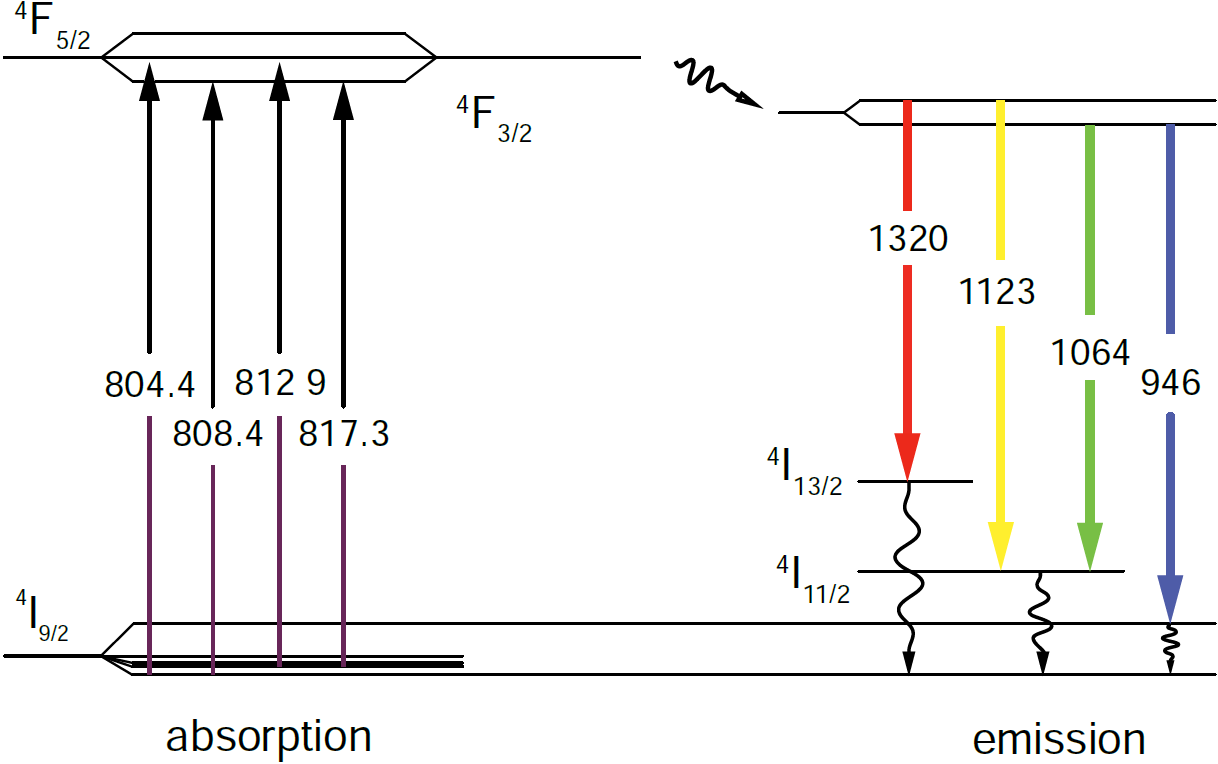
\includegraphics[width=\textwidth]{spectrum.png}
	\caption{Transitions in the Nd:YAG crystal \cite{lit:leybold}.}
	\label{fig:spectrum}
\end{figure}


\subsection{Nonlinear effect}
KTP crystal (Potassium titanyl phosphate, $\mathsf{K\,TiO\,PO_4}$)

two photon effect, quadratic

frequency doubling

energy conservation: $E = h \nu$
\begin{equation}
	\nu_2 = 2 \nu_1
\end{equation}

momentum conservation: $\vec p = \hbar \vec k$
\begin{equation}
	\vec k_2 = 2 \vec k_1
\end{equation}

$k = \frac{2 \pi}{\lambda}$
dispersion relation: $c = n c_0 = \lambda \nu$
\begin{equation}
2 = \frac{k_2}{k_1} = \frac{n_2 \nu_2}{n_1 \nu_1} = 2\;\frac{n_2}{n_1}
\end{equation}

Thus the refraction index of the material has to be the same for both wavelengths. As most materials show normal diffraction, i.e. $n(\lambda) \searrow$, 





% merge into literature:

% R. Willingale: \emph{lecture notes, Lasers and Quantum Optics}. University of Leicester 2007.\\
% \url{http://www.star.le.ac.uk/~zrw/courses/lect4313.html}
% crop image:
% http://www.star.le.ac.uk/~zrw/courses/lect4313_fig16.jpg

% http://www.atlas.uni-wuppertal.de/FP/anleitungen/fpI-09/diodenlaser.pdf


% !TeX encoding = UTF-8
% !TeX root = V6_SAXS.tex
% !TeX spellcheck = en_US

We generate $40\,\keV$ x-ray radiation via bremsstrahlung from electrons emitted by a titanate ($\mathsf{TiO_4}$) probe accelerated in a capacitor.

The setup consists of three measurement spots at which x-rays can be applied by opening a shutter for 1 hour (Guinier) or 2 hours (front \& back scattering) respectively.



% Guinier
As the high intensity of the unscattered beam could damage the film, it is only exposed for 3\,s during a pre-measurement to generate a line on the film denoting 0\,\degree. Thereafter, we switch to 'EXP' mode where the central beam is blocked. The border of the covered area is clearly visible on the film as a ridge in the background noise.



\begin{figure}[h]
	\centering
	\vspace{1ex}
	\def\svgwidth{0.5\textwidth}
W	\input{graphics/Guinier_angle.pdf_tex}
	\caption{Angle relation for the Guinier camera: $180\degree - \beta = 180\degree - 2 \alpha$}
	\label{fig:guinier_geom}
%	\vspace{-3em}
\end{figure}






First measurement
\begin{itemize}\itemsep-5pt
	\item front scattering: tape
	\item Guinier mode: reference crystal
	\item back scattering: sodium chloride crystal \textsf{NaCl}
\end{itemize}

Second measurement
\begin{itemize}\itemsep-5pt
	\item front scattering: silicon powder in tape
	\item Guinier mode: silicon powder
	\item back scattering: silicon wafer
\end{itemize}

Third measurement
\begin{itemize}\itemsep-5pt
	\item front scattering: stretched polymer
	\item Guinier mode: polymer
	\item back scattering: lithium fluoride crystal \textsf{LiF}
\end{itemize}


As seen in figure \ref{fig:guinier_geom}, the spectrum recorded on the Guinier camera isn't distorted as it would be for a planar detector -- the position on the film linearly corresponds to the scattering angle, making the method useful for large scattering angles. Due to the slanted incident beam, we measure only one radial profile of the scattering intensities (instead of seeing it mirrored on the incident beam). As the film covers about 270\,\degree and the incident beam is slanted by ca. 45\,\degree, we can detect diffracted beams up to approximately $\alpha_{max} =\tfrac12 \beta_{max} = \tfrac12 \cdt (\tfrac{270}{2}\,\degree + 2 \cdt 45\,\degree) \approx 110\,\degree$.

The exact calibration is done via a silicon sample. However, the silicon powder is mounted on sticky tape which introduces its own diffraction pattern. To discern these lines, we also measure a piece of tape by itself.




The edge of the beam stopper can be clearly seen at 16.5\,mm, below which the background intensity is massively reduced. The considerable differences in shape for the three curves were caused by two errors:
\begin{enumerate}
\item
For the reference crystal, the timer wasn't set correctly, leading to an exposure time of nearly 2 1/2 hours. As this increases the intensity of both data and background, it has little effect on our measurement.
\item
While transferring the film with the spectrum of the polymer, the film accidentally dropped out of the envelope and was exposed to sunlight. As the hitherto unexposed areas of the film are more sensitive, this reduces the contrast considerably.
\end{enumerate}



Silicon:
24.1 ?
% 36.5 is the tape ?
48.9
52.0
73.9 ?
81.6
85.6
96.7
101.4
119.0
131.4
151.1



Polymer:
20.3
36.9
39.1
41
43.4
51.9
62.1
68.2
70.1
71.5
73.9
80.7
91.1
94.6
98.6
133.8









\begin{figure}[h]
	\centering
	\def\svgwidth{0.5\textwidth}
	% This file was created by matlab2tikz.
% Minimal pgfplots version: 1.3
%
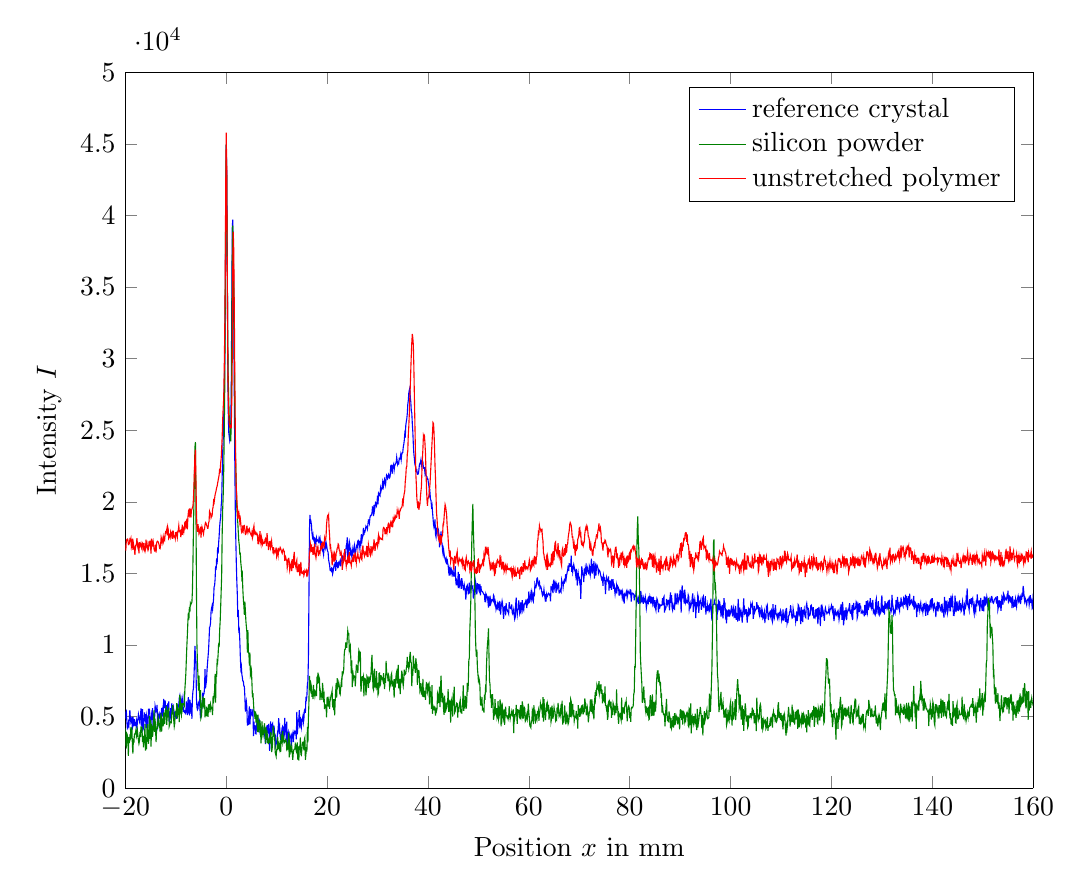
\begin{tikzpicture}

\begin{axis}[%
width=0.95092\textwidth,
height=0.75\textwidth,
at={(0\textwidth,0\textwidth)},
scale only axis,
separate axis lines,
xmin=-20,
xmax=160,
xlabel={Position $x$ in mm},
ymin=0,
ymax=50000,
ylabel={Intensity $I$},
legend style={legend cell align=left,align=left,draw=black}
]
\addplot [color=blue,solid]
  table[row sep=crcr]{%
-20	4865.6562\\
-19.9	5302.3438\\
-19.8	5372.7969\\
-19.7	4693.5\\
-19.6	4195.7031\\
-19.5	4280.6406\\
-19.4	4545.5\\
-19.3	4363.5\\
-19.2	4886.7188\\
-19.1	5456.8281\\
-19	4856.7344\\
-18.9	4605.6562\\
-18.8	4732.8906\\
-18.7	4971.6719\\
-18.6	4098.8125\\
-18.5	4999.4062\\
-18.4	4741.5312\\
-18.3	4326.2344\\
-18.2	4821.0156\\
-18.1	4496.1719\\
-18	4397.8906\\
-17.9	4463.0625\\
-17.8	4682.3594\\
-17.7	4087.5938\\
-17.6	4762.75\\
-17.5	4799.5469\\
-17.4	5165.8281\\
-17.3	4985.4531\\
-17.2	4618.9219\\
-17.1	4538.4844\\
-17	4999.7031\\
-16.9	5570.6406\\
-16.8	5089.2656\\
-16.7	4027.6406\\
-16.6	5522.3438\\
-16.5	4088.5781\\
-16.4	4189.2344\\
-16.3	4806.4844\\
-16.2	5306.0156\\
-16.1	4679\\
-16	5182.0156\\
-15.9	4220.2812\\
-15.8	5075.7344\\
-15.7	4876.5938\\
-15.6	4054.3438\\
-15.5	4558.9062\\
-15.4	5514.7812\\
-15.3	5533.4531\\
-15.2	5474.8906\\
-15.1	4875.1094\\
-15	4196.3594\\
-14.9	4638.0469\\
-14.8	5070.0312\\
-14.7	4780.4219\\
-14.6	5591.4062\\
-14.5	4269.6719\\
-14.4	5132.1406\\
-14.3	5031.9688\\
-14.2	4814.7812\\
-14.1	5760.1719\\
-14	5575.3281\\
-13.9	5378.7656\\
-13.8	5444.3438\\
-13.7	5821.6406\\
-13.6	4261.8281\\
-13.5	4383.9844\\
-13.4	5137.4219\\
-13.3	5242.5469\\
-13.2	4980.75\\
-13.1	4819.875\\
-13	5277.8125\\
-12.9	4906.4531\\
-12.8	5618.2969\\
-12.7	5196.875\\
-12.6	5464.8594\\
-12.5	5023.2188\\
-12.4	6236.2656\\
-12.3	5585.5\\
-12.2	6103.0781\\
-12.1	6096.0781\\
-12	5453.0938\\
-11.9	5811.0781\\
-11.8	5458.375\\
-11.7	5235.5156\\
-11.6	5934.7969\\
-11.5	5356.5469\\
-11.4	6069.5469\\
-11.3	4643.4219\\
-11.2	5016.5938\\
-11.1	4917.3906\\
-11	5589.7812\\
-10.9	5116.5625\\
-10.8	5932.7344\\
-10.7	5689.1875\\
-10.6	5597\\
-10.5	5719.4531\\
-10.4	5454.9531\\
-10.3	5025.7031\\
-10.2	5000.0625\\
-10.1	5331\\
-10	5340.3594\\
-9.9	4848.3125\\
-9.8	5724.4375\\
-9.7	5662.0938\\
-9.6	5787.0625\\
-9.5	5681.1094\\
-9.4	5801.9688\\
-9.3	6300.1719\\
-9.2	6460.3594\\
-9.1	5871.1562\\
-9	5649.3906\\
-8.9	6130.9688\\
-8.8	5876.5312\\
-8.7	6115.1094\\
-8.6	6328.2188\\
-8.5	5417.3594\\
-8.4	5466.0781\\
-8.3	5339.2344\\
-8.2	5384.7812\\
-8.1	5239.125\\
-8	5316.2969\\
-7.9	6073.9062\\
-7.8	5485.625\\
-7.7	5113.7656\\
-7.6	6032.9844\\
-7.5	6360.9219\\
-7.4	5218.75\\
-7.3	5168.5\\
-7.2	6194.6094\\
-7.1	5880.4688\\
-7	5198.7344\\
-6.9	5935.5938\\
-6.8	4841.5469\\
-6.7	6276.0625\\
-6.6	6770.7812\\
-6.5	6954.0625\\
-6.4	7695.9375\\
-6.3	8680.2812\\
-6.2	9945.7969\\
-6.1	9231.7344\\
-6	8898.9688\\
-5.9	6247.9219\\
-5.8	5662.2812\\
-5.7	5484.4844\\
-5.6	5553.9062\\
-5.5	6019.0938\\
-5.4	6019.8594\\
-5.3	6150.3125\\
-5.2	5504.3281\\
-5.1	4881.4375\\
-5	5198.5312\\
-4.9	5492.5469\\
-4.8	5598.5781\\
-4.7	6493.9844\\
-4.6	6363.5312\\
-4.5	6612.4219\\
-4.4	6603.4375\\
-4.3	6963.9062\\
-4.2	8314.5781\\
-4.1	6980.0312\\
-4	7289.125\\
-3.9	7521.9062\\
-3.8	8261.3125\\
-3.7	8757.2656\\
-3.6	9186.5\\
-3.5	9647.3281\\
-3.4	10391.4844\\
-3.3	11237.4062\\
-3.2	11302.0312\\
-3.1	11566.3594\\
-3	12352.3281\\
-2.9	12569.6875\\
-2.8	12740.6875\\
-2.7	12494.5312\\
-2.6	12845.2656\\
-2.5	13240.0156\\
-2.4	14087.0312\\
-2.3	14147.8281\\
-2.2	14604.5625\\
-2.1	15491.2656\\
-2	15247.0938\\
-1.9	16057.8594\\
-1.8	15638.0156\\
-1.7	16826.5625\\
-1.6	16386.1094\\
-1.5	17142.625\\
-1.4	17604.9531\\
-1.3	18261.6719\\
-1.2	18673.2031\\
-1.1	18910.2344\\
-1	19704.5938\\
-0.899999999999999	20128.6875\\
-0.799999999999997	21752.375\\
-0.699999999999999	23424.9219\\
-0.599999999999998	24319.4844\\
-0.5	25763.9219\\
-0.399999999999999	27391.875\\
-0.299999999999997	29570.2031\\
-0.199999999999999	33063.3438\\
-0.0999999999999979	39061.0156\\
0	44923.4844\\
0.100000000000001	43113.6094\\
0.200000000000003	37940.8438\\
0.300000000000001	30245.8594\\
0.400000000000002	26384.2969\\
0.5	24868.75\\
0.600000000000001	24536.1094\\
0.700000000000003	24275.4531\\
0.800000000000001	24496.9688\\
0.900000000000002	25185.1562\\
1	27772.7969\\
1.1	33467.3906\\
1.2	39102.1406\\
1.3	39709.625\\
1.4	37539.4219\\
1.5	32903.6719\\
1.6	27635.9219\\
1.7	23057.7969\\
1.8	19503.0156\\
1.9	17454.2812\\
2	15792.4844\\
2.1	14514.5469\\
2.2	13571.4844\\
2.3	11960.8281\\
2.4	12460.5625\\
2.5	10990.1094\\
2.6	11061.4531\\
2.7	10294.875\\
2.8	9176.0938\\
2.9	8366.4219\\
3	8534.5781\\
3.1	7957.5625\\
3.2	7740.3594\\
3.3	7478.7656\\
3.4	7461.9062\\
3.5	7135.4531\\
3.6	7119.3281\\
3.7	6404.1875\\
3.8	5363.0312\\
3.9	5709.6406\\
4	6016.375\\
4.1	5638.125\\
4.2	4369.3906\\
4.3	4877.0938\\
4.4	4409.3125\\
4.5	5223.9375\\
4.6	5711.0781\\
4.7	4454.8438\\
4.8	5102.5156\\
4.9	5520.7812\\
5	5189.4531\\
5.1	5091.7344\\
5.2	5177.625\\
5.3	5538.5469\\
5.4	3643.25\\
5.5	4647.7344\\
5.6	4103.5156\\
5.7	4406.2031\\
5.8	3826.0312\\
5.9	3798.1406\\
6	4302.6406\\
6.1	4647.4531\\
6.2	4153.0938\\
6.3	4149.125\\
6.4	4251.6094\\
6.5	4818.9375\\
6.6	4713.5625\\
6.7	3956.2656\\
6.8	4075.3125\\
6.9	4170.6406\\
7	4167.2656\\
7.1	4182.4844\\
7.2	4054.4219\\
7.3	4152.0781\\
7.4	3869.9062\\
7.5	3793.625\\
7.6	3800.2656\\
7.7	3458.2344\\
7.8	3081.2031\\
7.9	3499.3125\\
8	4166.9844\\
8.1	4050.0781\\
8.2	4408.9844\\
8.3	3819.3125\\
8.4	4489.4219\\
8.5	4083.5469\\
8.6	2613.0625\\
8.7	3334.2969\\
8.8	4672.8438\\
8.9	3737.7656\\
9	4101.625\\
9.1	4460.75\\
9.2	4528.0938\\
9.3	4013.3125\\
9.4	3666.0156\\
9.5	4368.375\\
9.6	3450.6406\\
9.7	3816\\
9.8	3024.8906\\
9.9	3212.125\\
10	3157.0938\\
10.1	3555.3906\\
10.2	3954.4531\\
10.3	4104.1875\\
10.4	4900.875\\
10.5	4072.7969\\
10.6	4269.1719\\
10.7	3643.7031\\
10.8	3418.0156\\
10.9	3424.6562\\
11	3915.8125\\
11.1	3644.5625\\
11.2	4307.1875\\
11.3	4246.6562\\
11.4	3502.7656\\
11.5	3708.9531\\
11.6	4921.1562\\
11.7	3906.4062\\
11.8	4498.125\\
11.9	3345.0312\\
12	4660.4531\\
12.1	2936.0469\\
12.2	3777.1875\\
12.3	3925.0938\\
12.4	3538.75\\
12.5	3313.125\\
12.6	3762.8438\\
12.7	3625.1406\\
12.8	3616.6875\\
12.9	2964.3438\\
13	3716.25\\
13.1	3619.1875\\
13.2	3811.7188\\
13.3	3220.4531\\
13.4	3754.1562\\
13.5	3955.9844\\
13.6	3863.6562\\
13.7	3953.5625\\
13.8	3882.125\\
13.9	3415.3125\\
14	5342.9844\\
14.1	3763.9062\\
14.2	4272.0781\\
14.3	4743.5469\\
14.4	4860.0625\\
14.5	5456.5\\
14.6	4187.9375\\
14.7	4985.5781\\
14.8	4561.375\\
14.9	4294.4844\\
15	4791.5469\\
15.1	4855.0469\\
15.2	5028.2656\\
15.3	4584.2344\\
15.4	4818.7969\\
15.5	5450.5\\
15.6	5516.1094\\
15.7	5274.8906\\
15.8	6262.5781\\
15.9	6191.8906\\
16	6446.1562\\
16.1	7347.6719\\
16.2	7456.3906\\
16.3	9059.0625\\
16.4	13199.5781\\
16.5	17937.8281\\
16.6	19082.625\\
16.7	18571.7188\\
16.8	18640.7188\\
16.9	18390.4844\\
17	17841.125\\
17.1	17569.0312\\
17.2	17727.7656\\
17.3	17395.875\\
17.4	17514.3906\\
17.5	17469.6406\\
17.6	16848.25\\
17.7	17301.2969\\
17.8	17189.2812\\
17.9	17482.4062\\
18	17288.6875\\
18.1	17332.25\\
18.2	17283.0781\\
18.3	17212\\
18.4	17453.5469\\
18.5	17277.75\\
18.6	17432.2812\\
18.7	16938.9844\\
18.8	17240.5781\\
18.9	17169.9844\\
19	17134.5156\\
19.1	16600.5781\\
19.2	16514.7969\\
19.3	16320.2031\\
19.4	16744.6406\\
19.5	16784.125\\
19.6	17022.5312\\
19.7	16827.1094\\
19.8	17177.875\\
19.9	17001.5\\
20	16717.5469\\
20.1	16553.1875\\
20.2	16493.5781\\
20.3	15973.9219\\
20.4	15764.0781\\
20.5	15576.3125\\
20.6	15236.4688\\
20.7	15257.6719\\
20.8	15186.5312\\
20.9	15387.75\\
21	15354.5312\\
21.1	14974.25\\
21.2	15138.4531\\
21.3	15401.1406\\
21.4	15572.9531\\
21.5	15519.9375\\
21.6	15785.5625\\
21.7	15181.2812\\
21.8	15938.4531\\
21.9	15458.25\\
22	15784.1719\\
22.1	15404.7188\\
22.2	15410.25\\
22.3	15724.2812\\
22.4	15629.0312\\
22.5	15797.8438\\
22.6	15908.6875\\
22.7	15503.8594\\
22.8	15895.9375\\
22.9	15871.6562\\
23	16260.5156\\
23.1	15833.9219\\
23.2	16139.8281\\
23.3	16118.9062\\
23.4	16145.25\\
23.5	16393.5469\\
23.6	16183.7969\\
23.7	16474.25\\
23.8	16938.75\\
23.9	17067.5156\\
24	17511.875\\
24.1	16136.3125\\
24.2	16318.9062\\
24.3	17008.5312\\
24.4	17242.1094\\
24.5	17069.5156\\
24.6	16244.625\\
24.7	16585.6094\\
24.8	16423.7812\\
24.9	16188.625\\
25	16659.4688\\
25.1	16392.5781\\
25.2	16506.1094\\
25.3	16752.9688\\
25.4	16952.9531\\
25.5	16453\\
25.6	16381.8281\\
25.7	16558.7188\\
25.8	16915.5312\\
25.9	16863.0938\\
26	17075.9375\\
26.1	16853.6562\\
26.2	17363.5625\\
26.3	17077.4062\\
26.4	17149.2656\\
26.5	16761.6406\\
26.6	17023.6875\\
26.7	17332.0938\\
26.8	17746.0781\\
26.9	17263.75\\
27	17531.0625\\
27.1	17562.5312\\
27.2	18189.4531\\
27.3	17684.75\\
27.4	17953.1406\\
27.5	17914.25\\
27.6	18055.9688\\
27.7	18295.2969\\
27.8	18215.0312\\
27.9	18256.625\\
28	18111.8125\\
28.1	18455.1406\\
28.2	18734.6875\\
28.3	18705.6406\\
28.4	18527.25\\
28.5	18896.2656\\
28.6	19047.7344\\
28.7	19032.8438\\
28.8	19088.7188\\
28.9	19209.3438\\
29	19636.9219\\
29.1	19599.4375\\
29.2	19002.7188\\
29.3	19779.7656\\
29.4	19415.5156\\
29.5	19645.2656\\
29.6	19939.0781\\
29.7	19880.9688\\
29.8	19740.4844\\
29.9	19964.2188\\
30	20427.625\\
30.1	19819.25\\
30.2	20613.2656\\
30.3	20550.625\\
30.4	20453.0312\\
30.5	20408.5156\\
30.6	20947.5625\\
30.7	20764.1719\\
30.8	20921.4219\\
30.9	21028.6562\\
31	21311.5781\\
31.1	20853.4062\\
31.2	21338.0312\\
31.3	21255.1875\\
31.4	21574.1875\\
31.5	21459.2656\\
31.6	21234.7188\\
31.7	21602.4688\\
31.8	21881\\
31.9	21824.4531\\
32	21617.7031\\
32.1	21692.5469\\
32.2	21903.0781\\
32.3	21800.4844\\
32.4	21685.3906\\
32.5	21767.7188\\
32.6	22381.9062\\
32.7	22272.1875\\
32.8	22603.4531\\
32.9	21959.4219\\
33	22518.4688\\
33.1	22523.2031\\
33.2	22632.2656\\
33.3	22228.7969\\
33.4	22508.2656\\
33.5	22600.7812\\
33.6	22691.0938\\
33.7	22751.3438\\
33.8	23114.2812\\
33.9	22845.75\\
34	22604.4531\\
34.1	22717.75\\
34.2	22669.6094\\
34.3	23018.8906\\
34.4	22990.1094\\
34.5	23112.8281\\
34.6	23307.8594\\
34.7	22973.6406\\
34.8	23301.5\\
34.9	23418.9219\\
35	23446.5\\
35.1	23810.6406\\
35.2	24008.4688\\
35.3	24272.2188\\
35.4	24716.7031\\
35.5	24484.1875\\
35.6	25320.125\\
35.7	25586.25\\
35.8	25792.125\\
35.9	26144.2188\\
36	26797.3594\\
36.1	27061.5312\\
36.2	27581.375\\
36.3	27788.9375\\
36.4	27945.1562\\
36.5	27305.0625\\
36.6	26971.3125\\
36.7	26338.8438\\
36.8	26204.5156\\
36.9	25437.2969\\
37	24891.9375\\
37.1	24015.8125\\
37.2	23375.2344\\
37.3	23050.1094\\
37.4	22648.4531\\
37.5	22504.3125\\
37.6	22347.3438\\
37.7	22143.7656\\
37.8	22194.8125\\
37.9	21933.3281\\
38	21926.5156\\
38.1	21974.6094\\
38.2	22219.0312\\
38.3	22585.1562\\
38.4	22685.1562\\
38.5	22735.3438\\
38.6	22925.2344\\
38.7	22529.0312\\
38.8	22720.5938\\
38.9	22882.0625\\
39	22780.7812\\
39.1	22352.9062\\
39.2	22369.7188\\
39.3	22385.0625\\
39.4	22040.9844\\
39.5	22255.2031\\
39.6	21869.2188\\
39.7	21769.6719\\
39.8	21756.5\\
39.9	21585.1094\\
40	21589.25\\
40.1	21263.8594\\
40.2	21087.8438\\
40.3	20501.0312\\
40.4	20647.0938\\
40.5	20192.4531\\
40.6	20100.6719\\
40.7	19697.4062\\
40.8	19808.4688\\
40.9	19308.0156\\
41	18882.375\\
41.1	18438.7656\\
41.2	18222.1719\\
41.3	18404.375\\
41.4	18768.0469\\
41.5	17732.5156\\
41.6	17549.8906\\
41.7	18113.9219\\
41.8	18061.9219\\
41.9	18158.2031\\
42	17802.7656\\
42.1	17945.2969\\
42.2	17603.7031\\
42.3	16829.0469\\
42.4	17337.7188\\
42.5	17579.1719\\
42.6	17934.5312\\
42.7	17168.9219\\
42.8	17112.1094\\
42.9	16579.9375\\
43	16346.1562\\
43.1	16656.5781\\
43.2	16352.4219\\
43.3	16174\\
43.4	16007.7656\\
43.5	15874.7344\\
43.6	16018.8438\\
43.7	15633.625\\
43.8	16032.8438\\
43.9	15720.5781\\
44	15580.4688\\
44.1	15178.2031\\
44.2	15431.8125\\
44.3	14845.8125\\
44.4	15382.8438\\
44.5	15266.4375\\
44.6	15018.25\\
44.7	15255.9688\\
44.8	15106.1562\\
44.9	14936.3906\\
45	15114.0625\\
45.1	14824.4531\\
45.2	14811.0469\\
45.3	14947.9375\\
45.4	15502.9688\\
45.5	14576.5469\\
45.6	14168.8125\\
45.7	14505.4062\\
45.8	14393.8125\\
45.9	14228.6094\\
46	15103.8438\\
46.1	13999.1562\\
46.2	14947.5781\\
46.3	14264.5312\\
46.4	14462.1406\\
46.5	14316.5938\\
46.6	13931.8438\\
46.7	14665\\
46.8	14426.8906\\
46.9	14150.2344\\
47	13925.9219\\
47.1	13870.4688\\
47.2	14195.7188\\
47.3	13976.1875\\
47.4	13927.8906\\
47.5	13184.2969\\
47.6	13622.875\\
47.7	14111.9375\\
47.8	14184.5625\\
47.9	14005.5781\\
48	13594.7812\\
48.1	13649.5469\\
48.2	14361.2969\\
48.3	13593.4688\\
48.4	13893.8594\\
48.5	13965.7188\\
48.6	14502.6406\\
48.7	13995\\
48.8	14080.3906\\
48.9	14116.2656\\
49	13253.5312\\
49.1	13834\\
49.2	13837.4219\\
49.3	13482.4844\\
49.4	14483.9219\\
49.5	14283.8438\\
49.6	13818.4688\\
49.7	13535.125\\
49.8	14318.9219\\
49.9	13890.3281\\
50	14262.5938\\
50.1	13797.5625\\
50.2	13730.1562\\
50.3	14278.2344\\
50.4	13477.6562\\
50.5	14120.4219\\
50.6	13772.5469\\
50.7	13763.6094\\
50.8	13740.5625\\
50.9	13670.9844\\
51	13605.1562\\
51.1	13538.125\\
51.2	13529.5469\\
51.3	12997.7812\\
51.4	13455.7969\\
51.5	13217.1094\\
51.6	13492.0469\\
51.7	13399.4844\\
51.8	13336.9688\\
51.9	13010.0938\\
52	12623.2188\\
52.1	13437.375\\
52.2	13139.5\\
52.3	12723.2812\\
52.4	13175.4219\\
52.5	12953.875\\
52.6	13081.6406\\
52.7	13171.7344\\
52.8	13157.6875\\
52.9	13086.75\\
53	13484.8906\\
53.1	13408.3281\\
53.2	12906.1719\\
53.3	12786.625\\
53.4	12965.0312\\
53.5	12515.0625\\
53.6	12690.4531\\
53.7	12592.9219\\
53.8	12860.0625\\
53.9	12655.8281\\
54	12917.0156\\
54.1	12977.0781\\
54.2	12371.4688\\
54.3	13040.5938\\
54.4	12123.2344\\
54.5	12677.1406\\
54.6	12838.7969\\
54.7	13080.4375\\
54.8	12883.5312\\
54.9	12281.125\\
55	11835.1875\\
55.1	12615.0469\\
55.2	12676.4531\\
55.3	12688.3125\\
55.4	12080.625\\
55.5	12934.9219\\
55.6	12462.2188\\
55.7	12476.1094\\
55.8	12341.9688\\
55.9	12296.4375\\
56	12184.8281\\
56.1	12993.4062\\
56.2	12747.5156\\
56.3	12585.5156\\
56.4	12545.1719\\
56.5	12536.6094\\
56.6	12831.25\\
56.7	12262.2188\\
56.8	12180.5156\\
56.9	12313\\
57	12488.7969\\
57.1	12073.2031\\
57.2	11802.7812\\
57.3	11942.1875\\
57.4	12901.0156\\
57.5	13317.2344\\
57.6	12404.3281\\
57.7	12109.25\\
57.8	12475.7031\\
57.9	12513.4375\\
58	13120.9062\\
58.1	12772.0938\\
58.2	12202.7812\\
58.3	12340.4375\\
58.4	12980.3594\\
58.5	12479.7656\\
58.6	12728.1562\\
58.7	13140.6562\\
58.8	12472.2969\\
58.9	12652.2812\\
59	12499.7656\\
59.1	12886.2969\\
59.2	12850.9219\\
59.3	12964.9688\\
59.4	13086.25\\
59.5	12962.3594\\
59.6	12581.6875\\
59.7	13231.4219\\
59.8	12889.9844\\
59.9	12964.1406\\
60	13754.9688\\
60.1	12990.7969\\
60.2	13034.5312\\
60.3	13346.875\\
60.4	13595.0469\\
60.5	13299.5625\\
60.6	13719.0781\\
60.7	13518.9688\\
60.8	13115.6562\\
60.9	13035.1094\\
61	13708.6094\\
61.1	13403.3438\\
61.2	14206.7656\\
61.3	14026.5781\\
61.4	14011.0938\\
61.5	14184.0156\\
61.6	14661.3281\\
61.7	14680.1406\\
61.8	14435.2344\\
61.9	14225.7031\\
62	14333.5469\\
62.1	14409.1875\\
62.2	14004.3438\\
62.3	14113.2812\\
62.4	14067.5469\\
62.5	13887.3594\\
62.6	13642.7188\\
62.7	13482.6719\\
62.8	13629.75\\
62.9	13560.6719\\
63	13881.6719\\
63.1	13549.9531\\
63.2	13292.4688\\
63.3	13557.7812\\
63.4	13027.7656\\
63.5	13522.0469\\
63.6	13359.7031\\
63.7	13413.5156\\
63.8	13558.1562\\
63.9	13619.4375\\
64	13578.0625\\
64.1	13506.7969\\
64.2	13549.0625\\
64.3	13060.0469\\
64.4	14049.8125\\
64.5	14007.3438\\
64.6	13895.3594\\
64.7	14267.25\\
64.8	13624.5625\\
64.9	14455.4219\\
65	14388.8281\\
65.1	14061.1406\\
65.2	14404.7344\\
65.3	14300.1406\\
65.4	13638.625\\
65.5	14141.4375\\
65.6	13901.3594\\
65.7	13992.3906\\
65.8	14281.3438\\
65.9	14312.125\\
66	13641.6562\\
66.1	13651.3906\\
66.2	13726.9531\\
66.3	13860.3594\\
66.4	13759.4219\\
66.5	14538.4531\\
66.6	14377.1875\\
66.7	14387.4531\\
66.8	14059.5781\\
66.9	14397.7812\\
67	14515.6562\\
67.1	14401.4688\\
67.2	14534.2969\\
67.3	14941.4375\\
67.4	14633.8594\\
67.5	14890.7656\\
67.6	15084.2188\\
67.7	15241.3438\\
67.8	15569.3906\\
67.9	15171.8594\\
68	15678.7812\\
68.1	15661.1406\\
68.2	15495.9531\\
68.3	15506.25\\
68.4	16236.9531\\
68.5	15106.2344\\
68.6	15545.1406\\
68.7	15122.875\\
68.8	15395.8594\\
68.9	15617.4531\\
69	15444.75\\
69.1	15217.3438\\
69.2	15129.4219\\
69.3	14855.1562\\
69.4	15321.3594\\
69.5	15025.3906\\
69.6	14162.2344\\
69.7	14526.7812\\
69.8	14984.8906\\
69.9	14702.2656\\
70	14722.3125\\
70.1	14339.0938\\
70.2	14433.6719\\
70.3	13232.8281\\
70.4	14422.9688\\
70.5	15485.4844\\
70.6	15164.5938\\
70.7	14929.7031\\
70.8	14855.7812\\
70.9	14398.6875\\
71	15349.5625\\
71.1	14842.4531\\
71.2	15379.2344\\
71.3	15139.0469\\
71.4	15021.3125\\
71.5	15529.2344\\
71.6	15411.1406\\
71.7	15157.9375\\
71.8	15029.9219\\
71.9	14978.4219\\
72	15526.4219\\
72.1	15403.7656\\
72.2	14954.2031\\
72.3	15240.1406\\
72.4	16029.2656\\
72.5	15274.6875\\
72.6	14988.5469\\
72.7	15672.625\\
72.8	15155.875\\
72.9	15857.7656\\
73	14634.4062\\
73.1	15257.9375\\
73.2	15476.5312\\
73.3	14850.4844\\
73.4	15453.5312\\
73.5	15595.7656\\
73.6	15498.1719\\
73.7	15353.2031\\
73.8	15064.0312\\
73.9	15255.6719\\
74	15203.375\\
74.1	15139.1719\\
74.2	14959.6562\\
74.3	14801.1719\\
74.4	14614.7031\\
74.5	14738.3594\\
74.6	14718.2969\\
74.7	14127.25\\
74.8	14867.1875\\
74.9	14698.1719\\
75	14697.0312\\
75.1	14347.3594\\
75.2	13553.2812\\
75.3	14294.8438\\
75.4	14692.0781\\
75.5	14516.6406\\
75.6	14495.375\\
75.7	14427.5781\\
75.8	14795.6094\\
75.9	13801.5469\\
76	14509.3438\\
76.1	13977.4375\\
76.2	14352.875\\
76.3	14452.0625\\
76.4	13851.2344\\
76.5	14587.3906\\
76.6	14153.7344\\
76.7	14597.2656\\
76.8	13923.8594\\
76.9	14309.9844\\
77	13879.2031\\
77.1	13561.1094\\
77.2	13861.6562\\
77.3	13753.7344\\
77.4	14144.8281\\
77.5	13855.3438\\
77.6	14126.0156\\
77.7	14054.9688\\
77.8	13960.0312\\
77.9	13443.2344\\
78	13796.5312\\
78.1	13726.5469\\
78.2	13621.3594\\
78.3	13814.7031\\
78.4	13761.3281\\
78.5	13388.9062\\
78.6	13666.3594\\
78.7	13337.5938\\
78.8	13577.7344\\
78.9	12887.7656\\
79	13543.7031\\
79.1	13478.1719\\
79.2	13456.7188\\
79.3	13693.75\\
79.4	13785.5156\\
79.5	13332.3438\\
79.6	13510.5469\\
79.7	13744.0938\\
79.8	13664.0312\\
79.9	13644.7656\\
80	13596.0938\\
80.1	13862.3281\\
80.2	13828.6875\\
80.3	13040.8906\\
80.4	13448.5938\\
80.5	13624.625\\
80.6	13580.75\\
80.7	13600.4531\\
80.8	13557.1406\\
80.9	13132.5469\\
81	13444.2344\\
81.1	13397.9688\\
81.2	13427.875\\
81.3	13797\\
81.4	12967.6719\\
81.5	13165.0781\\
81.6	13093.1406\\
81.7	13370.6719\\
81.8	12876.6406\\
81.9	13507\\
82	12975.5625\\
82.1	12953.6875\\
82.2	13774.7031\\
82.3	13407.0938\\
82.4	13012.9062\\
82.5	13022.5312\\
82.6	13262.3281\\
82.7	12880.0156\\
82.8	13222.1562\\
82.9	13042.8438\\
83	13017.625\\
83.1	13324.7031\\
83.2	13050.0625\\
83.3	12583.3125\\
83.4	12836.7656\\
83.5	13104.8438\\
83.6	12936.5625\\
83.7	12904.8438\\
83.8	13427.25\\
83.9	13012.8594\\
84	13348.5156\\
84.1	13117.1562\\
84.2	13395.0938\\
84.3	12915.4375\\
84.4	13366.5312\\
84.5	12980.75\\
84.6	13294.875\\
84.7	13321.2656\\
84.8	12761.1406\\
84.9	12691.4844\\
85	13128.5469\\
85.1	12599.9844\\
85.2	12427.4375\\
85.3	12921.8281\\
85.4	13241.2188\\
85.5	13134\\
85.6	12925.2344\\
85.7	12286.2812\\
85.8	12854.9844\\
85.9	12857.2812\\
86	12663.625\\
86.1	12795.7344\\
86.2	12775.7969\\
86.3	12762.4219\\
86.4	12799.7812\\
86.5	13267.3281\\
86.6	12795.7656\\
86.7	13286.4688\\
86.8	13377.9531\\
86.9	12262.1875\\
87	12637.2969\\
87.1	12536.1562\\
87.2	12640.0938\\
87.3	13166.2188\\
87.4	13140.0469\\
87.5	12892.9688\\
87.6	13075.8906\\
87.7	13111.4219\\
87.8	12803.875\\
87.9	12430.2656\\
88	13353.0469\\
88.1	13681.5781\\
88.2	12939.625\\
88.3	13488.8281\\
88.4	12580.7969\\
88.5	12439.7188\\
88.6	12795.6094\\
88.7	12647.2812\\
88.8	12550.6094\\
88.9	12512.2344\\
89	13643.0938\\
89.1	13114.2344\\
89.2	12881.4844\\
89.3	12882.8594\\
89.4	13627.8438\\
89.5	13161.9375\\
89.6	12972.1562\\
89.7	13138.1562\\
89.8	13406.9531\\
89.9	13283.5625\\
90	13873.0469\\
90.1	13355.7031\\
90.2	12275.1406\\
90.3	13611.9219\\
90.4	14172.2812\\
90.5	13465.875\\
90.6	13633.2656\\
90.7	13370.5781\\
90.8	12898.7031\\
90.9	13874.9844\\
91	13499.125\\
91.1	12982.875\\
91.2	13134.25\\
91.3	12990.5\\
91.4	12951.7656\\
91.5	13088.1406\\
91.6	13496.9219\\
91.7	13385.8125\\
91.8	12506.4844\\
91.9	12717.8281\\
92	12915.3594\\
92.1	12691.6562\\
92.2	12836.0781\\
92.3	12934.2188\\
92.4	13350.8438\\
92.5	13609.25\\
92.6	12306.7031\\
92.7	13040.6562\\
92.8	12900.7656\\
92.9	13178.5\\
93	12933.4688\\
93.1	11875\\
93.2	13003.8281\\
93.3	12641.0781\\
93.4	12770.9219\\
93.5	13509.375\\
93.6	13365.7812\\
93.7	12241.8281\\
93.8	12860.5938\\
93.9	13037.8906\\
94	12981.7188\\
94.1	13143.5938\\
94.2	12463.5781\\
94.3	12714.9375\\
94.4	12757.2969\\
94.5	13342.6094\\
94.6	13414.0312\\
94.7	12585.4375\\
94.8	12890.2188\\
94.9	12848.8281\\
95	13409.5625\\
95.1	12120.8281\\
95.2	12722.4062\\
95.3	12367.8906\\
95.4	12789.0312\\
95.5	12535.0469\\
95.6	12647.5781\\
95.7	12444.625\\
95.8	12704.0312\\
95.9	12501.8906\\
96	12739.8906\\
96.1	13235.0312\\
96.2	12252.1094\\
96.3	11707.3594\\
96.4	12252.7188\\
96.5	12812.6719\\
96.6	12823.5156\\
96.7	12822.8594\\
96.8	13053.2344\\
96.9	12860\\
97	12851.0156\\
97.1	12839.6094\\
97.2	12420.9531\\
97.3	11752.5938\\
97.4	12637.4531\\
97.5	12511.9531\\
97.6	13082.5781\\
97.7	13002.4688\\
97.8	12429.6562\\
97.9	12830.3438\\
98	12578.8438\\
98.1	11990.1094\\
98.2	12475.7812\\
98.3	12294.9219\\
98.4	12798.4062\\
98.5	11865.1875\\
98.6	12561.0469\\
98.7	13274.1406\\
98.8	12732.2656\\
98.9	12816.875\\
99	12043.0625\\
99.1	12210.0312\\
99.2	11511.6719\\
99.3	12374.9688\\
99.4	12316.2656\\
99.5	11990.7812\\
99.6	12481.5938\\
99.7	11994.7031\\
99.8	12465.4531\\
99.9	12137.0781\\
100	12249.6406\\
100.1	12419.9219\\
100.2	12765.9531\\
100.3	12324.9219\\
100.4	11998.6562\\
100.5	12448.7812\\
100.6	12616.3594\\
100.7	12093.1875\\
100.8	12252.375\\
100.9	11885.5938\\
101	12736.4219\\
101.1	11768.7969\\
101.2	12192.1719\\
101.3	12154.9844\\
101.4	11644.125\\
101.5	13219.6562\\
101.6	12642.7656\\
101.7	11683.4062\\
101.8	12619.2188\\
101.9	12376.0156\\
102	12127.25\\
102.1	12310.2969\\
102.2	12065.4219\\
102.3	11566.9531\\
102.4	12277.7031\\
102.5	12459.1406\\
102.6	13257.3906\\
102.7	12286.4219\\
102.8	12477.1094\\
102.9	12179.0781\\
103	12200.4688\\
103.1	12501.4062\\
103.2	12055.375\\
103.3	11566.6406\\
103.4	12217.2656\\
103.5	12408.4844\\
103.6	11998.5938\\
103.7	12562.1875\\
103.8	12172\\
103.9	12206.9531\\
104	12830.6875\\
104.1	12667.2656\\
104.2	12752.8594\\
104.3	12900.9375\\
104.4	12500.9219\\
104.5	11837.5938\\
104.6	12180.2031\\
104.7	12737.8594\\
104.8	12312.3125\\
104.9	12422.25\\
105	12487.9219\\
105.1	12529.8594\\
105.2	12990.25\\
105.3	12638.1406\\
105.4	12752.4531\\
105.5	12723.0938\\
105.6	12288.8125\\
105.7	12119.6406\\
105.8	12643.4062\\
105.9	12339.1875\\
106	12191.9062\\
106.1	11930.5781\\
106.2	12556.125\\
106.3	12403.5625\\
106.4	11841.4375\\
106.5	11896.8594\\
106.6	12158.1406\\
106.7	12325.7656\\
106.8	11539.9219\\
106.9	12180.8125\\
107	11836.1406\\
107.1	12611.6719\\
107.2	12456.6875\\
107.3	12668.9688\\
107.4	12107.0781\\
107.5	11741.6562\\
107.6	12168.5156\\
107.7	12228.375\\
107.8	12311.2656\\
107.9	12059.9375\\
108	12331.9375\\
108.1	12426.3906\\
108.2	11754.2344\\
108.3	11624.2656\\
108.4	12849.5938\\
108.5	12059.8594\\
108.6	12279.9531\\
108.7	11972.8594\\
108.8	12250.7656\\
108.9	12804.2812\\
109	12186.4062\\
109.1	12151.1562\\
109.2	12005.1406\\
109.3	11879.5469\\
109.4	12225.125\\
109.5	12227.5781\\
109.6	11944.25\\
109.7	12210.9375\\
109.8	12140.0781\\
109.9	12420.1562\\
110	12318.9375\\
110.1	11785.0312\\
110.2	11979.0938\\
110.3	11860.2812\\
110.4	12491.6406\\
110.5	11711.2969\\
110.6	11945.6875\\
110.7	12023.6094\\
110.8	12216.3125\\
110.9	11614.8438\\
111	12217.7969\\
111.1	12586.2656\\
111.2	11516.7188\\
111.3	11682.1562\\
111.4	11638.0781\\
111.5	12046.2812\\
111.6	12067.1406\\
111.7	12323.125\\
111.8	12338.2031\\
111.9	12788.6406\\
112	12395.0781\\
112.1	12072.5938\\
112.2	11881.7969\\
112.3	11930.875\\
112.4	12531.8594\\
112.5	12296.9531\\
112.6	11986.4219\\
112.7	12013.1875\\
112.8	12015.5938\\
112.9	11651.2188\\
113	11983.9062\\
113.1	12341.375\\
113.2	11673.6406\\
113.3	12006.9219\\
113.4	12819.0625\\
113.5	12758.0781\\
113.6	12245.75\\
113.7	12413.2031\\
113.8	12125.4531\\
113.9	11466.0312\\
114	12644.0938\\
114.1	11683.2969\\
114.2	12462.6094\\
114.3	11602.5469\\
114.4	12355.9688\\
114.5	12277.9844\\
114.6	12490.4219\\
114.7	12132.1719\\
114.8	11975.7969\\
114.9	11920.25\\
115	12733.9844\\
115.1	12903.6562\\
115.2	12612.7969\\
115.3	12530.1562\\
115.4	11772.3438\\
115.5	12295.1562\\
115.6	12039.9375\\
115.7	12057.2031\\
115.8	12161.3906\\
115.9	12743.3906\\
116	12789.9062\\
116.1	12580.4219\\
116.2	12376.7188\\
116.3	12054.1094\\
116.4	12643.4219\\
116.5	11911.8281\\
116.6	11940.8125\\
116.7	11897.8438\\
116.8	12283.8125\\
116.9	12116.5312\\
117	12500.5469\\
117.1	11988.0938\\
117.2	12582.0469\\
117.3	11469.5312\\
117.4	11978.5469\\
117.5	12669.4062\\
117.6	12379.4531\\
117.7	12053.6406\\
117.8	11329.5312\\
117.9	12479.0781\\
118	12826.0938\\
118.1	11951.6875\\
118.2	12615.3906\\
118.3	12465.9688\\
118.4	12244.0312\\
118.5	12003.2656\\
118.6	11692.8906\\
118.7	12393.2969\\
118.8	12587.3125\\
118.9	12382.6094\\
119	12308.5938\\
119.1	12199.3438\\
119.2	12282.5469\\
119.3	12259.1719\\
119.4	12331.2031\\
119.5	12571.75\\
119.6	12264.625\\
119.7	12424.1562\\
119.8	12506.4531\\
119.9	12601.2969\\
120	12764.0156\\
120.1	12546.3281\\
120.2	12365.4844\\
120.3	12735.6719\\
120.4	12116.7969\\
120.5	11677.8438\\
120.6	12013.6719\\
120.7	12556.4531\\
120.8	12256.0156\\
120.9	12130.4531\\
121	12222.5781\\
121.1	12095.1719\\
121.2	12317.9062\\
121.3	12397.2188\\
121.4	12154.0781\\
121.5	11777.5781\\
121.6	12041.8281\\
121.7	12378.5469\\
121.8	12135.1562\\
121.9	12834.5312\\
122	12366.75\\
122.1	11761.4062\\
122.2	13011.1562\\
122.3	12500.1094\\
122.4	11372.5938\\
122.5	11824.4688\\
122.6	12413.7344\\
122.7	12046.4531\\
122.8	12284.9531\\
122.9	12636.6875\\
123	11743.4219\\
123.1	12201.5625\\
123.2	12325.3281\\
123.3	12473.2344\\
123.4	12432.7344\\
123.5	12665.3906\\
123.6	12929.4062\\
123.7	12246.0469\\
123.8	12225.0312\\
123.9	12334.1094\\
124	12132.9219\\
124.1	12791.1719\\
124.2	11751.3906\\
124.3	12590.8438\\
124.4	12948.4062\\
124.5	12473.5781\\
124.6	12488.3281\\
124.7	12519.7812\\
124.8	12641.8594\\
124.9	13015.6875\\
125	12923.9219\\
125.1	11891.0625\\
125.2	12038.4688\\
125.3	12849.4688\\
125.4	12731.8125\\
125.5	12294.9844\\
125.6	12920.2344\\
125.7	12621.4219\\
125.8	12659.8438\\
125.9	12257.8125\\
126	12298.7656\\
126.1	12238.2812\\
126.2	12381.4531\\
126.3	12310.0938\\
126.4	12272.4062\\
126.5	12011.6875\\
126.6	12795.1875\\
126.7	12457.8125\\
126.8	12095.0469\\
126.9	13062.3906\\
127	12426.9688\\
127.1	12253.5625\\
127.2	13120.9844\\
127.3	12451.0469\\
127.4	12786.6875\\
127.5	12906.4531\\
127.6	12774.4688\\
127.7	13283.4375\\
127.8	12829.7812\\
127.9	12636.4219\\
128	12963.0938\\
128.1	12538.4531\\
128.2	13154.1562\\
128.3	12306.5\\
128.4	12402.3906\\
128.5	12227.6406\\
128.6	12367.1719\\
128.7	12225.9531\\
128.8	13082.8906\\
128.9	13234.1094\\
129	12161.5\\
129.1	12748.8594\\
129.2	12487.2031\\
129.3	13060.6406\\
129.4	12070.4219\\
129.5	12659.8438\\
129.6	12143.2656\\
129.7	12240.2344\\
129.8	12256\\
129.9	13112.2344\\
130	13461.6719\\
130.1	12370.6562\\
130.2	12332.5781\\
130.3	12686.8281\\
130.4	12641.9062\\
130.5	12129.5781\\
130.6	13059\\
130.7	12530.2969\\
130.8	12892.125\\
130.9	12870.1562\\
131	12613.1094\\
131.1	12842.7969\\
131.2	12668.25\\
131.3	13123\\
131.4	12519.6094\\
131.5	13176.0312\\
131.6	12594.1562\\
131.7	12554.8281\\
131.8	12302.4062\\
131.9	12450.5\\
132	13510.0625\\
132.1	12882.5625\\
132.2	12708.9844\\
132.3	12239.2812\\
132.4	12440.6094\\
132.5	12309.1719\\
132.6	12205.3125\\
132.7	12456.6562\\
132.8	13130.4844\\
132.9	12476.8438\\
133	12948.4531\\
133.1	13366.2188\\
133.2	12677.2969\\
133.3	12815.4844\\
133.4	12576.7188\\
133.5	12400.2031\\
133.6	13033.4688\\
133.7	12665.2188\\
133.8	13324.8594\\
133.9	12840.6094\\
134	12935.0781\\
134.1	12815.3594\\
134.2	12708.2656\\
134.3	13285.7188\\
134.4	13208.1562\\
134.5	12801.9375\\
134.6	13228.75\\
134.7	13513.2031\\
134.8	12940.4688\\
134.9	13139.7031\\
135	12715.4531\\
135.1	12449.7969\\
135.2	13415.8125\\
135.3	13169.2188\\
135.4	12974.2344\\
135.5	13590.6094\\
135.6	12848.75\\
135.7	12897.0625\\
135.8	13101.25\\
135.9	13154.7031\\
136	12977.5156\\
136.1	12809.3125\\
136.2	12751.3125\\
136.3	13441.0625\\
136.4	12473.2188\\
136.5	13030.6875\\
136.6	12985.2969\\
136.7	12699.7188\\
136.8	12772.8125\\
136.9	11959.1562\\
137	12801.5625\\
137.1	12336.4062\\
137.2	12897.0625\\
137.3	12883.375\\
137.4	12662.875\\
137.5	12414.6875\\
137.6	12741.5312\\
137.7	12938.6719\\
137.8	12569.1719\\
137.9	12447.2188\\
138	12543.0625\\
138.1	12322.2969\\
138.2	12894.5156\\
138.3	12556.2188\\
138.4	12684.5312\\
138.5	12938.2656\\
138.6	12359.5312\\
138.7	12044.6094\\
138.8	12791.3594\\
138.9	12604.5156\\
139	12847.9688\\
139.1	12093.9062\\
139.2	12647.8906\\
139.3	12724.125\\
139.4	12438.2656\\
139.5	12490.9844\\
139.6	13077.5312\\
139.7	13138.1562\\
139.8	12686.0312\\
139.9	12837.6094\\
140	13280.8281\\
140.1	12647.8906\\
140.2	12493.3281\\
140.3	12846.6719\\
140.4	12887.9219\\
140.5	12560.4844\\
140.6	12470.5469\\
140.7	11957.7969\\
140.8	12720.9688\\
140.9	12400.4219\\
141	13035.0938\\
141.1	12347.1875\\
141.2	12616.7969\\
141.3	13002.8906\\
141.4	12673.4375\\
141.5	12641.6719\\
141.6	12449.4531\\
141.7	12535.0625\\
141.8	12869.0938\\
141.9	12265.5625\\
142	12634.0781\\
142.1	12397.7031\\
142.2	12257.0469\\
142.3	11922.1406\\
142.4	13370.8594\\
142.5	12476.2344\\
142.6	12335.875\\
142.7	13107.8125\\
142.8	12626.375\\
142.9	12819.3594\\
143	12226.4375\\
143.1	12412.2188\\
143.2	13027.6562\\
143.3	12591.9844\\
143.4	13283.1094\\
143.5	12396.4688\\
143.6	12393.3906\\
143.7	13453.1094\\
143.8	12648.8281\\
143.9	13149.0781\\
144	13319.1562\\
144.1	12607.9844\\
144.2	12072.9531\\
144.3	12062.7031\\
144.4	12433.0781\\
144.5	13449.9844\\
144.6	12908.625\\
144.7	12298.3906\\
144.8	12674.7969\\
144.9	13044.0625\\
145	12549.0312\\
145.1	12625.8906\\
145.2	12379\\
145.3	13013.7812\\
145.4	13061.1875\\
145.5	12466.3125\\
145.6	12926.9844\\
145.7	12344.6406\\
145.8	12412.0625\\
145.9	12718.5469\\
146	13040.4219\\
146.1	12744.9062\\
146.2	12543.8125\\
146.3	12058.4062\\
146.4	12740.6719\\
146.5	12531.8438\\
146.6	12600\\
146.7	13242.125\\
146.8	13076.7969\\
146.9	13950.1406\\
147	13155.875\\
147.1	12729.9062\\
147.2	12652.6094\\
147.3	12450.1406\\
147.4	13212.5156\\
147.5	12899.7031\\
147.6	12926.0781\\
147.7	13281.1562\\
147.8	12911.4844\\
147.9	13167.1719\\
148	13265.4219\\
148.1	12867.6719\\
148.2	12397.8594\\
148.3	12178.0312\\
148.4	12721.2188\\
148.5	12506.4688\\
148.6	12342.0625\\
148.7	13120.6094\\
148.8	12699.5156\\
148.9	13536.6562\\
149	13047.6406\\
149.1	12961.0781\\
149.2	12849.8281\\
149.3	13116.75\\
149.4	12353\\
149.5	12892.7344\\
149.6	13296.9844\\
149.7	12759.7812\\
149.8	12635.1094\\
149.9	12395.6094\\
150	13150.25\\
150.1	12887.8594\\
150.2	12362.9062\\
150.3	13361.8125\\
150.4	13356.0156\\
150.5	12762.2031\\
150.6	13136.4062\\
150.7	13010.4688\\
150.8	13374.8125\\
150.9	13173.0938\\
151	12660.3281\\
151.1	13224.9219\\
151.2	12589.4062\\
151.3	12360.3906\\
151.4	13201.1875\\
151.5	13117.3594\\
151.6	13054.7031\\
151.7	13387.7344\\
151.8	13394.3594\\
151.9	13137.0781\\
152	12972.6094\\
152.1	12924.8594\\
152.2	13005.8281\\
152.3	13192.5781\\
152.4	13213.9531\\
152.5	13275.6094\\
152.6	13314.5156\\
152.7	12963.5469\\
152.8	12919.3125\\
152.9	13408.2656\\
153	12478.9062\\
153.1	12678.4688\\
153.2	13124.4219\\
153.3	12632.7188\\
153.4	13070.3125\\
153.5	13051.5781\\
153.6	12387.8906\\
153.7	12775.4062\\
153.8	13385.8438\\
153.9	13310.0938\\
154	12823.1094\\
154.1	13603.4688\\
154.2	13517.6562\\
154.3	13176.5625\\
154.4	13330.2031\\
154.5	13247.25\\
154.6	13139.0938\\
154.7	13145.4531\\
154.8	13424.9219\\
154.9	13345.5\\
155	13801.6094\\
155.1	13017.1719\\
155.2	13098.2969\\
155.3	13411.7031\\
155.4	13367.3438\\
155.5	12973.0312\\
155.6	13289.4531\\
155.7	13252.4062\\
155.8	12585.5781\\
155.9	13414.125\\
156	12840.6719\\
156.1	12719.5156\\
156.2	12854.6562\\
156.3	13173.7969\\
156.4	12661.0312\\
156.5	13199.25\\
156.6	12974.5781\\
156.7	12704.5312\\
156.8	13088.3594\\
156.9	13261.125\\
157	13413.4844\\
157.1	13107.6719\\
157.2	13282.3906\\
157.3	13112.4531\\
157.4	13290.2656\\
157.5	12863\\
157.6	13452.9219\\
157.7	13163.7188\\
157.8	13652.5\\
157.9	13366.3281\\
158	14131.3906\\
158.1	13849.0469\\
158.2	13341.3125\\
158.3	13070.1719\\
158.4	13280.3125\\
158.5	13179.375\\
158.6	12961.8594\\
158.7	12814.5469\\
158.8	13089.2344\\
158.9	13179.4219\\
159	13130.3438\\
159.1	13233.0781\\
159.2	12816.5156\\
159.3	13089.7188\\
159.4	13483.9531\\
159.5	12928.5938\\
159.6	13190.5781\\
159.7	13088.625\\
159.8	12548.5781\\
159.9	12613.1875\\
160	13587.75\\
};
\addlegendentry{reference crystal};

\addplot [color=black!50!green,solid]
  table[row sep=crcr]{%
-20	4187.9663\\
-19.9	3055.7119\\
-19.8	2948.0339\\
-19.7	3811.4746\\
-19.6	3720.2881\\
-19.5	3408.1694\\
-19.4	2261.1355\\
-19.3	3572.4067\\
-19.2	3148.2034\\
-19.1	3599.7627\\
-19	3513.4746\\
-18.9	4282.729\\
-18.8	3462.6948\\
-18.7	4253.6611\\
-18.6	3033.6101\\
-18.5	2416.3389\\
-18.4	3466.8813\\
-18.3	3165.9153\\
-18.2	3767.1187\\
-18.1	3801.4238\\
-18	3861.2542\\
-17.9	4082.1865\\
-17.8	3588.9321\\
-17.7	3704.2542\\
-17.6	4014.7288\\
-17.5	3676.1355\\
-17.4	3336.2373\\
-17.3	3119.5762\\
-17.2	3291.1865\\
-17.1	3931.9832\\
-17	3571.9321\\
-16.9	4318.627\\
-16.8	3868.678\\
-16.7	4286.6104\\
-16.6	3249.7966\\
-16.5	3648.5933\\
-16.4	2853.0339\\
-16.3	3190.3052\\
-16.2	3601.5593\\
-16.1	4477.9829\\
-16	2625.4575\\
-15.9	3156.1355\\
-15.8	2727.0847\\
-15.7	4188.2036\\
-15.6	4476.1357\\
-15.5	3390.4575\\
-15.4	3112.7795\\
-15.3	3715.2542\\
-15.2	5063.5762\\
-15.1	3457.0508\\
-15	4791.9321\\
-14.9	2909.0339\\
-14.8	4405.5083\\
-14.7	4318.1016\\
-14.6	3584.1526\\
-14.5	4021.1187\\
-14.4	4565.8306\\
-14.3	5452.729\\
-14.2	3940.0847\\
-14.1	4859.6948\\
-14	3988.3728\\
-13.9	3230.644\\
-13.8	4071.3899\\
-13.7	4366.2036\\
-13.6	4145.8813\\
-13.5	5000.9829\\
-13.4	4836.5591\\
-13.3	4416.1865\\
-13.2	4359.5254\\
-13.1	3926.0508\\
-13	4876.5591\\
-12.9	5242.356\\
-12.8	3951.6101\\
-12.7	4616.2544\\
-12.6	4883.7119\\
-12.5	4320.085\\
-12.4	5295.8813\\
-12.3	4828.729\\
-12.2	4476.3389\\
-12.1	5451.6611\\
-12	5032.2202\\
-11.9	5742.6104\\
-11.8	4424.7119\\
-11.7	4961.1016\\
-11.6	5475\\
-11.5	4958.9829\\
-11.4	5631.2881\\
-11.3	4326.5591\\
-11.2	4442.729\\
-11.1	4614.915\\
-11	4659.8306\\
-10.9	4608.0679\\
-10.8	5161.271\\
-10.7	5402.2036\\
-10.6	5804.2881\\
-10.5	5240.4238\\
-10.4	4742.9492\\
-10.3	4319.5591\\
-10.2	4528.2544\\
-10.1	5222.3896\\
-10	5066.5762\\
-9.9	5089\\
-9.8	5938.8306\\
-9.7	4866.9663\\
-9.6	5629.0171\\
-9.5	5472.1016\\
-9.4	5416.0508\\
-9.3	4613.0171\\
-9.2	6522.7627\\
-9.1	6213\\
-9	5344.1523\\
-8.9	5130.0679\\
-8.8	5942.1357\\
-8.7	5569.356\\
-8.6	5889.0679\\
-8.5	5874.3896\\
-8.4	5917.8984\\
-8.3	5801.356\\
-8.2	6875.0679\\
-8.1	7433.6777\\
-8	8037.0171\\
-7.9	9016.7793\\
-7.8	9946.3389\\
-7.7	10715.4238\\
-7.6	11611.0674\\
-7.5	12267.1016\\
-7.4	11776.4238\\
-7.3	12655.8643\\
-7.2	12311.542\\
-7.1	12926.0508\\
-7	12834.3223\\
-6.9	12921.9834\\
-6.8	12987.1523\\
-6.7	13758.2373\\
-6.6	15615.2539\\
-6.5	17950.8301\\
-6.4	19928.2031\\
-6.3	21717.5078\\
-6.2	23824.7793\\
-6.1	24176.7285\\
-6	19672.5938\\
-5.9	13973.3555\\
-5.8	10005\\
-5.7	8717.9658\\
-5.6	7868.627\\
-5.5	6815.627\\
-5.4	7862.7119\\
-5.3	6726.7456\\
-5.2	6159.4746\\
-5.1	6855.9321\\
-5	4917.271\\
-4.9	5048.1523\\
-4.8	5609.5933\\
-4.7	6120.8984\\
-4.6	6406.6611\\
-4.5	5758.3052\\
-4.4	5880.0508\\
-4.3	6286.1523\\
-4.2	4948.8643\\
-4.1	5323.2373\\
-4	5197.8813\\
-3.9	5702.8984\\
-3.8	5054.271\\
-3.7	5615.4409\\
-3.6	4980.356\\
-3.5	5864.5083\\
-3.4	5470.7798\\
-3.3	5886.6611\\
-3.2	5310.373\\
-3.1	5854.8643\\
-3	5681.627\\
-2.9	5604.729\\
-2.8	5480.3389\\
-2.7	5118.3389\\
-2.6	6428.1357\\
-2.5	5926.2881\\
-2.4	6526.729\\
-2.3	6829.4067\\
-2.2	7980.9663\\
-2.1	5984.5762\\
-2	7992.5591\\
-1.9	7785.1694\\
-1.8	8888.542\\
-1.7	8802.5928\\
-1.6	9369.8984\\
-1.5	10117.458\\
-1.4	9856.1182\\
-1.3	11036.8135\\
-1.2	11626.2881\\
-1.1	12622.5254\\
-1	13743.9834\\
-0.899999999999999	14829.8301\\
-0.799999999999997	17693.5078\\
-0.699999999999999	19461.7637\\
-0.599999999999998	20406.9492\\
-0.5	22028.5078\\
-0.399999999999999	24461.627\\
-0.299999999999997	27569.4922\\
-0.199999999999999	33102.6797\\
-0.0999999999999979	41205.4922\\
0	44967.4062\\
0.100000000000001	42767.7969\\
0.200000000000003	37026.5078\\
0.300000000000001	31765.1016\\
0.400000000000002	28621.2891\\
0.5	27198.2715\\
0.600000000000001	25947.2207\\
0.700000000000003	25311.8145\\
0.800000000000001	24454.5254\\
0.900000000000002	24230.2891\\
1	25370.9668\\
1.1	30056.2363\\
1.2	37050.4414\\
1.3	39295.4727\\
1.4	37847.3555\\
1.5	34445.3203\\
1.6	30167.8301\\
1.7	26843.1348\\
1.8	23928.1016\\
1.9	22411.5078\\
2	21097.7285\\
2.1	19610.7285\\
2.2	18984.5254\\
2.3	18528.0176\\
2.4	17857.4062\\
2.5	17255.7793\\
2.6	16953.3555\\
2.7	16362.1523\\
2.8	16383.3223\\
2.9	15721.9326\\
3	15395.4404\\
3.1	14718.8477\\
3.2	14891.2031\\
3.3	13868.5928\\
3.4	13191.1865\\
3.5	12763.6611\\
3.6	12108.3223\\
3.7	13039.1523\\
3.8	12411.3896\\
3.9	11690.9658\\
4	11280.0508\\
4.1	10897.6953\\
4.2	9471.8643\\
4.3	11039.2881\\
4.4	9512.1699\\
4.5	9389.1016\\
4.6	8562.3555\\
4.7	9462.8301\\
4.8	7884.271\\
4.9	8014.9829\\
5	8220.8477\\
5.1	7380.5933\\
5.2	6356.0337\\
5.3	6633.9492\\
5.4	6015.2373\\
5.5	5402.7119\\
5.6	5363.3896\\
5.7	4846.1523\\
5.8	5364.729\\
5.9	4579.373\\
6	5091.4238\\
6.1	4997.3052\\
6.2	3917.1187\\
6.3	5142.9829\\
6.4	4278.8813\\
6.5	3910.7795\\
6.6	4324.2373\\
6.7	4743.1523\\
6.8	4223.4067\\
6.9	3142.2034\\
7	3813.2034\\
7.1	4677.3052\\
7.2	3889.5762\\
7.3	3648.6611\\
7.4	3875.5085\\
7.5	4267.271\\
7.6	4536.729\\
7.7	3849.1694\\
7.8	3135.2712\\
7.9	4260.2036\\
8	3388.322\\
8.1	4036.1355\\
8.2	3144.2542\\
8.3	3541.356\\
8.4	3157.7966\\
8.5	3211.1187\\
8.6	3447.1865\\
8.7	3307.2034\\
8.8	3865.3899\\
8.9	3842.1694\\
9	2527.0339\\
9.1	2728.4575\\
9.2	3176.9832\\
9.3	4350.8477\\
9.4	4100.8813\\
9.5	3686.1355\\
9.6	3724.1187\\
9.7	2524.7458\\
9.8	2393.4746\\
9.9	2235.4915\\
10	2689.5593\\
10.1	2744.5085\\
10.2	3593.0508\\
10.3	2888.3899\\
10.4	3054.9321\\
10.5	2794.9832\\
10.6	2671.2034\\
10.7	3340.3052\\
10.8	2542.1865\\
10.9	3614.322\\
11	3417.2542\\
11.1	3227.356\\
11.2	3989.7119\\
11.3	3400.8474\\
11.4	3515.9661\\
11.5	3177.644\\
11.6	3225.8474\\
11.7	3308.1526\\
11.8	3394.4915\\
11.9	3313.8982\\
12	2751.2034\\
12.1	2856.3899\\
12.2	2759.5085\\
12.3	3495.7627\\
12.4	3885.7966\\
12.5	2151.0339\\
12.6	3153.7966\\
12.7	2944.0339\\
12.8	2558.3389\\
12.9	2699.6272\\
13	2918.1355\\
13.1	2436.6272\\
13.2	1988.0509\\
13.3	2493.2034\\
13.4	2669.2205\\
13.5	2733.2205\\
13.6	2736.2373\\
13.7	3100.7966\\
13.8	3009.8306\\
13.9	2573.9832\\
14	2485.7288\\
14.1	3198.3389\\
14.2	1988.339\\
14.3	2926.1865\\
14.4	1937.9491\\
14.5	2961.356\\
14.6	2697.5593\\
14.7	3544.5933\\
14.8	2367.3728\\
14.9	2319.7627\\
15	2715.3728\\
15.1	3121.4915\\
15.2	3224.5933\\
15.3	3225.6611\\
15.4	2649.4915\\
15.5	3429.3389\\
15.6	3547.2542\\
15.7	1977.9491\\
15.8	2362.8982\\
15.9	2867.0168\\
16	2563.4575\\
16.1	4287.6104\\
16.2	3211.2712\\
16.3	4945.627\\
16.4	5966.4067\\
16.5	7849.3223\\
16.6	7311.0337\\
16.7	6946.373\\
16.8	7281.5933\\
16.9	7095.4575\\
17	6389.7119\\
17.1	6798.4067\\
17.2	6235.7119\\
17.3	7221\\
17.4	6413.7798\\
17.5	6904.5933\\
17.6	6490.2036\\
17.7	6740.1187\\
17.8	6659.1523\\
17.9	6433.2036\\
18	7798.373\\
18.1	7589.7627\\
18.2	8078.271\\
18.3	7322.4917\\
18.4	7766.0337\\
18.5	7641.6611\\
18.6	6163.356\\
18.7	6715.2036\\
18.8	6474.5762\\
18.9	6539.7964\\
19	6183.4067\\
19.1	7359.356\\
19.2	6911.8643\\
19.3	6309.2202\\
19.4	6497.1357\\
19.5	5532.1187\\
19.6	5782.5425\\
19.7	5814.4746\\
19.8	5728.9829\\
19.9	4945.4067\\
20	6365.1016\\
20.1	6053.8813\\
20.2	6398.4238\\
20.3	5698.5425\\
20.4	6106.4409\\
20.5	5552.8813\\
20.6	6298.8813\\
20.7	6245.1694\\
20.8	6522.2544\\
20.9	6611.8135\\
21	6802.4917\\
21.1	5659.3052\\
21.2	6216.644\\
21.3	5467.6777\\
21.4	6220.4575\\
21.5	5090\\
21.6	6036.3896\\
21.7	6728.1016\\
21.8	7341.4409\\
21.9	6324.3896\\
22	7693.8306\\
22.1	7057.3223\\
22.2	7176.6104\\
22.3	7384.8984\\
22.4	7181.6948\\
22.5	6640.5083\\
22.6	6555.3052\\
22.7	7003.1523\\
22.8	7340.7798\\
22.9	7077.5933\\
23	8166.7627\\
23.1	7932.8306\\
23.2	8049.1694\\
23.3	8309.1357\\
23.4	9335.2881\\
23.5	9683.1865\\
23.6	9708.1357\\
23.7	10144.4072\\
23.8	10134.3223\\
23.9	9803.0674\\
24	10448.6445\\
24.1	10999.8135\\
24.2	10759.8135\\
24.3	10777.7119\\
24.4	9631.5762\\
24.5	9813.6953\\
24.6	9948.085\\
24.7	9109.1016\\
24.8	8043.5933\\
24.9	8926.4238\\
25	7072.8813\\
25.1	8235.1523\\
25.2	7657.8477\\
25.3	7867.5254\\
25.4	7836.0679\\
25.5	7803.6777\\
25.6	7119.4409\\
25.7	7885.0679\\
25.8	8586.0342\\
25.9	8549.0342\\
26	8375.1016\\
26.1	8053.4238\\
26.2	9013.6445\\
26.3	9630.915\\
26.4	9517.8984\\
26.5	8808.8984\\
26.6	9532.915\\
26.7	6743.644\\
26.8	7039.2036\\
26.9	7772.627\\
27	7790.8813\\
27.1	7621.8984\\
27.2	7785.2544\\
27.3	6421.1187\\
27.4	7719.3052\\
27.5	7267.7456\\
27.6	7668.1016\\
27.7	6490.7456\\
27.8	6873.271\\
27.9	7814.3052\\
28	7727.5425\\
28.1	7375.4238\\
28.2	7012\\
28.3	7819.3389\\
28.4	7405.4409\\
28.5	7466.2202\\
28.6	7687.3223\\
28.7	7930.4746\\
28.8	8749.3047\\
28.9	9308.8301\\
29	8151.3896\\
29.1	7005.7964\\
29.2	6879.2881\\
29.3	7980.356\\
29.4	8349.7119\\
29.5	7116.8643\\
29.6	7149.4575\\
29.7	7028.373\\
29.8	8174.1694\\
29.9	7019.2202\\
30	7360.0337\\
30.1	6533.3052\\
30.2	6656.2881\\
30.3	8023.271\\
30.4	8042.3389\\
30.5	7165.6948\\
30.6	7253.7627\\
30.7	7899.373\\
30.8	7638.3389\\
30.9	7704.1357\\
31	7618.4575\\
31.1	7480\\
31.2	8030.085\\
31.3	7588.1694\\
31.4	6918.9492\\
31.5	7690.4917\\
31.6	7356.2036\\
31.7	8896.6777\\
31.8	8130.644\\
31.9	7982.2373\\
32	7822.4917\\
32.1	7459.9829\\
32.2	7888.7798\\
32.3	7746.356\\
32.4	6994.0337\\
32.5	7149.7119\\
32.6	7327.8643\\
32.7	7901.6777\\
32.8	8017\\
32.9	7094.7964\\
33	7389.2036\\
33.1	7470.8306\\
33.2	7075.729\\
33.3	6329.5933\\
33.4	7618.1523\\
33.5	7031.3896\\
33.6	7541.4238\\
33.7	7987.5254\\
33.8	8134.0679\\
33.9	7317.6948\\
34	7605.4238\\
34.1	8610.458\\
34.2	6973.7119\\
34.3	7634.0337\\
34.4	7368.1357\\
34.5	6577.8643\\
34.6	7514.271\\
34.7	7446.5591\\
34.8	8218.2539\\
34.9	7968.8477\\
35	7411.1865\\
35.1	7167.1357\\
35.2	7567.0508\\
35.3	8281.1699\\
35.4	7924.8984\\
35.5	7965.1187\\
35.6	8014.2373\\
35.7	8324.7119\\
35.8	8568.3389\\
35.9	9172.5596\\
36	8435.9492\\
36.1	8805.9492\\
36.2	8341.0508\\
36.3	8513.9492\\
36.4	9246.7793\\
36.5	9524.8477\\
36.6	8831.542\\
36.7	8769.5762\\
36.8	7125.7119\\
36.9	8097.7798\\
37	7872.7627\\
37.1	9269.0342\\
37.2	8712.2207\\
37.3	8480.5762\\
37.4	8577.6953\\
37.5	8066.1357\\
37.6	9090.2539\\
37.7	8694.627\\
37.8	8633.9834\\
37.9	7224.915\\
38	8287.5254\\
38.1	7710.4067\\
38.2	8253.5254\\
38.3	7573.8135\\
38.4	6865.4067\\
38.5	7076.6777\\
38.6	7343.1694\\
38.7	6544.2881\\
38.8	7096.7119\\
38.9	6402.0337\\
39	7643.2544\\
39.1	6373.1016\\
39.2	6692.2544\\
39.3	6374.8813\\
39.4	6799.5425\\
39.5	6171.1187\\
39.6	6943.4067\\
39.7	7363.4067\\
39.8	7324.8984\\
39.9	6724.644\\
40	6904.5254\\
40.1	7248.2881\\
40.2	7333.1357\\
40.3	5860.915\\
40.4	7099.8643\\
40.5	6371.3896\\
40.6	6749.9492\\
40.7	5540.5083\\
40.8	7198.6104\\
40.9	5205.5254\\
41	5761.2881\\
41.1	5643.6104\\
41.2	5539.8813\\
41.3	5643.5254\\
41.4	5469.8477\\
41.5	5070.8306\\
41.6	5510.6948\\
41.7	5394.9321\\
41.8	5552.6948\\
41.9	6625.9492\\
42	6484.5591\\
42.1	5949.4575\\
42.2	6418.9829\\
42.3	7097.2202\\
42.4	5662.3052\\
42.5	7141.1865\\
42.6	7863.8306\\
42.7	6572.8643\\
42.8	6001.8306\\
42.9	6665.3896\\
43	6265.6104\\
43.1	5476.4238\\
43.2	5130.8813\\
43.3	6464.271\\
43.4	5273.0171\\
43.5	5691.4067\\
43.6	5860.4067\\
43.7	5641.5762\\
43.8	5942.7119\\
43.9	5968.2036\\
44	6924.085\\
44.1	5344.8643\\
44.2	6181.2881\\
44.3	5633.8477\\
44.4	5831.4746\\
44.5	4577.2373\\
44.6	5996.9321\\
44.7	6173.7627\\
44.8	5668.4746\\
44.9	5002.7964\\
45	6357.2202\\
45.1	6187.4917\\
45.2	7102.2036\\
45.3	5292.4238\\
45.4	5378.2036\\
45.5	5642.4067\\
45.6	5729.3389\\
45.7	5943.4238\\
45.8	5905.3052\\
45.9	4941.5425\\
46	5679.5591\\
46.1	5346.3389\\
46.2	5798.1865\\
46.3	5992.9492\\
46.4	6162.356\\
46.5	5346.6948\\
46.6	5257.085\\
46.7	5249.7964\\
46.8	5718.9663\\
46.9	6165.5425\\
47	7189.271\\
47.1	5413.3389\\
47.2	5954.4575\\
47.3	5791.8306\\
47.4	6442.4746\\
47.5	6183.9492\\
47.6	5558.0171\\
47.7	6077\\
47.8	7355.5425\\
47.9	6741.4409\\
48	7269.6104\\
48.1	8920.627\\
48.2	9109.7793\\
48.3	11102.5928\\
48.4	11961.458\\
48.5	13159.9326\\
48.6	15243.373\\
48.7	17375\\
48.8	18721.9824\\
48.9	19850.084\\
49	18132.2207\\
49.1	16975.8809\\
49.2	15919\\
49.3	13336.1865\\
49.4	10878.373\\
49.5	9769.3555\\
49.6	9181.3389\\
49.7	9678.7119\\
49.8	8430.373\\
49.9	7999.4067\\
50	7519.8135\\
50.1	7690.0679\\
50.2	7526.6948\\
50.3	7158.4917\\
50.4	5866.8813\\
50.5	5808.0337\\
50.6	5828.2202\\
50.7	6387.1523\\
50.8	5483.1016\\
50.9	5523.4067\\
51	5570.0171\\
51.1	5278.8813\\
51.2	6532.3052\\
51.3	6182.9492\\
51.4	6913.2202\\
51.5	6701.4746\\
51.6	8471.4238\\
51.7	9422.1182\\
51.8	10105.8301\\
51.9	10444.0342\\
52	11171.3555\\
52.1	9293.9658\\
52.2	7503.6104\\
52.3	7271.3896\\
52.4	6289.1694\\
52.5	6552.8477\\
52.6	5610.4409\\
52.7	6297.0679\\
52.8	6565.4067\\
52.9	5872.9492\\
53	4787.4575\\
53.1	5081.2373\\
53.2	5116.085\\
53.3	6228.6611\\
53.4	5314.5083\\
53.5	5194.5933\\
53.6	5590.0679\\
53.7	4899.271\\
53.8	5026.4575\\
53.9	6086.5083\\
54	4815.8135\\
54.1	4988\\
54.2	5314.5762\\
54.3	6207.0508\\
54.4	5693.7119\\
54.5	4330.0679\\
54.6	5116.8135\\
54.7	5971.5933\\
54.8	5382.2036\\
54.9	4815.8135\\
55	5045.8984\\
55.1	5505.1357\\
55.2	4429.6948\\
55.3	5179.5083\\
55.4	5692.271\\
55.5	5075.5254\\
55.6	5066.6948\\
55.7	4950.9829\\
55.8	5011.6948\\
55.9	4831.6948\\
56	4995.1357\\
56.1	5734.1523\\
56.2	5207.1523\\
56.3	4863.5083\\
56.4	5091.0679\\
56.5	5114.1865\\
56.6	5333.7456\\
56.7	5090.7119\\
56.8	5044.085\\
56.9	5508.3389\\
57	3854.5933\\
57.1	5173.9492\\
57.2	4897.2881\\
57.3	5137.7964\\
57.4	5177.9321\\
57.5	5823.644\\
57.6	5103.2544\\
57.7	4497.4575\\
57.8	5484.1187\\
57.9	5466.915\\
58	5405.5762\\
58.1	5142.1187\\
58.2	5363.6948\\
58.3	4812.2036\\
58.4	5796.6611\\
58.5	5241.2544\\
58.6	5031.9321\\
58.7	6064.2373\\
58.8	5765.2036\\
58.9	4868.5083\\
59	5100.7456\\
59.1	5640.2373\\
59.2	5576.3223\\
59.3	4681.4746\\
59.4	4757.7798\\
59.5	5001.9492\\
59.6	5167.0679\\
59.7	4874.2544\\
59.8	5184.5083\\
59.9	5917\\
60	5314.2036\\
60.1	4922.3896\\
60.2	4357.9663\\
60.3	4302.7119\\
60.4	4229.9663\\
60.5	4682.1523\\
60.6	4724.2881\\
60.7	5478.7119\\
60.8	5361.1694\\
60.9	4485.4917\\
61	5812.4067\\
61.1	5021.7456\\
61.2	5490.7627\\
61.3	4513.4746\\
61.4	5195.8984\\
61.5	4930.7798\\
61.6	4803.7456\\
61.7	5306.7627\\
61.8	5258.2202\\
61.9	5437.2881\\
62	4714.0508\\
62.1	5247.3896\\
62.2	5426.3389\\
62.3	5926.9663\\
62.4	5735.8813\\
62.5	5604.8477\\
62.6	5852.6104\\
62.7	4927.4746\\
62.8	6367.5762\\
62.9	4650.4238\\
63	6219.5254\\
63.1	5594.627\\
63.2	5175.085\\
63.3	4759.5591\\
63.4	5382.4746\\
63.5	5768.7964\\
63.6	5564.4067\\
63.7	5872.7119\\
63.8	5577.1187\\
63.9	5814.915\\
64	4795.5762\\
64.1	5103.4238\\
64.2	5370.1865\\
64.3	5651\\
64.4	4642.8477\\
64.5	4853.8135\\
64.6	5765.6777\\
64.7	5249.9663\\
64.8	4872.6948\\
64.9	5233.085\\
65	5652.729\\
65.1	5394.4238\\
65.2	5336.4746\\
65.3	4717.7627\\
65.4	4799.2373\\
65.5	4756.2036\\
65.6	5643.7627\\
65.7	5210.0508\\
65.8	5967\\
65.9	5381.6777\\
66	5010.3896\\
66.1	5085.915\\
66.2	5339.4575\\
66.3	5136.8135\\
66.4	5870.8813\\
66.5	5155.356\\
66.6	6112.3223\\
66.7	4444.8643\\
66.8	4640.8306\\
66.9	4628.4917\\
67	5157\\
67.1	5790.2881\\
67.2	5161.9492\\
67.3	4468.1357\\
67.4	5142.2036\\
67.5	5234.5254\\
67.6	4750.4917\\
67.7	4911.356\\
67.8	4502.0171\\
67.9	4607.6104\\
68	4954.8135\\
68.1	5993.1357\\
68.2	4976.4746\\
68.3	6198.1357\\
68.4	6062.1357\\
68.5	5173.4409\\
68.6	5342.0171\\
68.7	5899.1016\\
68.8	5012.5254\\
68.9	5457.8984\\
69	4699.2036\\
69.1	4921.9663\\
69.2	4999.6777\\
69.3	4959.5591\\
69.4	5407.4575\\
69.5	4809.5762\\
69.6	5185.2373\\
69.7	4159.4067\\
69.8	5801.6948\\
69.9	5233.4575\\
70	5350.1187\\
70.1	4989.5933\\
70.2	5413.0508\\
70.3	5256.5762\\
70.4	5570.7964\\
70.5	5399.6948\\
70.6	5779.2881\\
70.7	5805.8306\\
70.8	5169.6948\\
70.9	5633.5591\\
71	5309.7798\\
71.1	6273.2202\\
71.2	5951.4238\\
71.3	5909.0508\\
71.4	5088.373\\
71.5	5382.2202\\
71.6	5614.8477\\
71.7	5266.9321\\
71.8	4609.7627\\
71.9	5004.4409\\
72	5318.3223\\
72.1	5411.9829\\
72.2	6211.5425\\
72.3	5665.4746\\
72.4	5334.1016\\
72.5	6221.5083\\
72.6	5430.5254\\
72.7	5641.0679\\
72.8	5373.5425\\
72.9	4806.3896\\
73	5961.1187\\
73.1	6389.5762\\
73.2	6175.2036\\
73.3	6873.7456\\
73.4	6458.9492\\
73.5	7183.271\\
73.6	7006.2036\\
73.7	7109.0508\\
73.8	6917.1865\\
73.9	7486.1694\\
74	6586.085\\
74.1	6790.9492\\
74.2	7209.5591\\
74.3	7223.6104\\
74.4	6592.915\\
74.5	6885.356\\
74.6	5938.8984\\
74.7	6645.2036\\
74.8	6411\\
74.9	6112.1865\\
75	6046.5762\\
75.1	7114.6777\\
75.2	5797.9829\\
75.3	5766.4746\\
75.4	5519.9829\\
75.5	5649.3052\\
75.6	4773.8643\\
75.7	5016.6104\\
75.8	5952.3223\\
75.9	5836.2202\\
76	6053.1016\\
76.1	5897.5254\\
76.2	5715\\
76.3	6046.3223\\
76.4	4913.644\\
76.5	5626.8813\\
76.6	5115.085\\
76.7	5958.8984\\
76.8	5825.7627\\
76.9	5767.5591\\
77	5093.7456\\
77.1	5345.0679\\
77.2	5755.8306\\
77.3	5249.4917\\
77.4	6909.1694\\
77.5	5463.1357\\
77.6	5727.356\\
77.7	4934.6948\\
77.8	4500.4917\\
77.9	5178.6948\\
78	5069.8477\\
78.1	5145.6104\\
78.2	4934.1523\\
78.3	4765.2036\\
78.4	6335.627\\
78.5	4754.9829\\
78.6	5571.2544\\
78.7	5619.7627\\
78.8	5590.1865\\
78.9	5189.5762\\
79	5676.8984\\
79.1	5923.2202\\
79.2	5857.8813\\
79.3	6082.0679\\
79.4	5496.1694\\
79.5	4677.3052\\
79.6	5318.4238\\
79.7	5649.2202\\
79.8	5738.8306\\
79.9	5627.373\\
80	4897.6611\\
80.1	5310.2544\\
80.2	4638.271\\
80.3	5564.3896\\
80.4	5648.1187\\
80.5	5615.8813\\
80.6	5670.729\\
80.7	5780.3389\\
80.8	6580.3052\\
80.9	6717.4067\\
81	8485.1357\\
81.1	8476.6445\\
81.2	10909\\
81.3	13617.1523\\
81.4	16463.1348\\
81.5	18128.3906\\
81.6	18980.5254\\
81.7	17371.084\\
81.8	16718.1523\\
81.9	15359.6953\\
82	13130.2715\\
82.1	9421.6104\\
82.2	8620.5596\\
82.3	7953.9663\\
82.4	7325.6948\\
82.5	5960.8643\\
82.6	6727.2881\\
82.7	6219.0171\\
82.8	7115.3223\\
82.9	5964.7456\\
83	6285.2881\\
83.1	5535.8306\\
83.2	5306.7456\\
83.3	5712.5762\\
83.4	5269.3896\\
83.5	5608.8984\\
83.6	5049.1694\\
83.7	5708.5254\\
83.8	4789.8135\\
83.9	4834.2373\\
84	6013.3223\\
84.1	6494.5933\\
84.2	5973.5425\\
84.3	5047.8984\\
84.4	5762.5762\\
84.5	6557.2881\\
84.6	5059.8984\\
84.7	6029.9663\\
84.8	5070.8643\\
84.9	5531.2881\\
85	6044.6104\\
85.1	5352.4575\\
85.2	5818.4409\\
85.3	7289.8984\\
85.4	7905.2544\\
85.5	8199.5254\\
85.6	8203.7969\\
85.7	7407.9829\\
85.8	8001.5591\\
85.9	7549.4917\\
86	7251.6104\\
86.1	7318.5591\\
86.2	6432.2036\\
86.3	6501.9829\\
86.4	5278.1694\\
86.5	5812.1865\\
86.6	5344.7456\\
86.7	5162.8813\\
86.8	5175.8813\\
86.9	5044.0679\\
87	4321.729\\
87.1	5206.2881\\
87.2	5668.915\\
87.3	6235.2202\\
87.4	5092.4238\\
87.5	4700.8135\\
87.6	5049.085\\
87.7	4607.0337\\
87.8	5361.8813\\
87.9	5098.271\\
88	4914.1865\\
88.1	4185.5425\\
88.2	4897.373\\
88.3	4201.2202\\
88.4	4332.0679\\
88.5	4532.0679\\
88.6	5035.1694\\
88.7	4240.9663\\
88.8	4760.5254\\
88.9	5241.8813\\
89	4417.3223\\
89.1	4681.356\\
89.2	5076.2202\\
89.3	4950.6777\\
89.4	4874.5591\\
89.5	4467.8984\\
89.6	4939.7456\\
89.7	4885.3223\\
89.8	4594.8135\\
89.9	4108.3389\\
90	5454.9321\\
90.1	5481.8135\\
90.2	5366.1016\\
90.3	4782.8984\\
90.4	5440.3389\\
90.5	4454.356\\
90.6	5263.5591\\
90.7	5339\\
90.8	5239.1523\\
90.9	4711.085\\
91	4937.5933\\
91.1	4764.373\\
91.2	5103.1523\\
91.3	5227.8306\\
91.4	5100.7798\\
91.5	5237.2881\\
91.6	4386.8643\\
91.7	4304.7627\\
91.8	5568.7627\\
91.9	5510.5425\\
92	4402.4067\\
92.1	5933.271\\
92.2	3842.4915\\
92.3	4773.2036\\
92.4	4985.4067\\
92.5	4668.2202\\
92.6	4507.0508\\
92.7	5031.2373\\
92.8	4722.4746\\
92.9	4572.2373\\
93	5209.9663\\
93.1	4765.0337\\
93.2	4491.5933\\
93.3	4063.2205\\
93.4	5536.4575\\
93.5	4234.2881\\
93.6	4551.4409\\
93.7	4728.0679\\
93.8	5124.3052\\
93.9	5325.5762\\
94	5678.5762\\
94.1	5316.085\\
94.2	4998.1357\\
94.3	4201.5425\\
94.4	5104.4409\\
94.5	3686.7288\\
94.6	4731.4746\\
94.7	4648.1694\\
94.8	5385.8813\\
94.9	4688.6104\\
95	4865.6948\\
95.1	5214.373\\
95.2	5291.4067\\
95.3	5483.8984\\
95.4	4855.627\\
95.5	4848.9492\\
95.6	4925.4238\\
95.7	4949.356\\
95.8	6601.4067\\
95.9	5946.9829\\
96	5339.5254\\
96.1	6177.0337\\
96.2	7294.8306\\
96.3	8399.8135\\
96.4	10798.3223\\
96.5	13461.5088\\
96.6	17100.9492\\
96.7	17380.4062\\
96.8	15123.4404\\
96.9	14043.1699\\
97	14164.2715\\
97.1	13350.627\\
97.2	11879.8818\\
97.3	9483.9658\\
97.4	7919.6948\\
97.5	7562.4746\\
97.6	6374.7627\\
97.7	5319.0337\\
97.8	5704.9829\\
97.9	5837.2881\\
98	6387.4409\\
98.1	6722.6104\\
98.2	5539.2881\\
98.3	5560.8477\\
98.4	5774.8135\\
98.5	6002.3389\\
98.6	5428\\
98.7	4931.6948\\
98.8	5442.0679\\
98.9	4937.1694\\
99	5483.7964\\
99.1	5531.3223\\
99.2	4401.0337\\
99.3	4569.4409\\
99.4	4866.2881\\
99.5	5483.373\\
99.6	4784.3896\\
99.7	4674.1016\\
99.8	5138.4917\\
99.9	5814.4238\\
100	6015.2373\\
100.1	4761.7798\\
100.2	5103.9321\\
100.3	4377.1016\\
100.4	6071.0508\\
100.5	5395.7456\\
100.6	4795.3223\\
100.7	5238.8984\\
100.8	5320.356\\
100.9	6223.7798\\
101	4766.5591\\
101.1	5198.2202\\
101.2	6430\\
101.3	7089.8477\\
101.4	7614.915\\
101.5	7014.3896\\
101.6	6728.9321\\
101.7	5564.3896\\
101.8	5716.271\\
101.9	6549.356\\
102	5657.1016\\
102.1	4800.8984\\
102.2	5319.4238\\
102.3	5779.5933\\
102.4	4431.7627\\
102.5	5525.3052\\
102.6	4009.322\\
102.7	4843.2202\\
102.8	5309.1694\\
102.9	5918.4746\\
103	5573.0679\\
103.1	4661.4575\\
103.2	5002.5591\\
103.3	5028.1187\\
103.4	4243.0679\\
103.5	4350.0337\\
103.6	4994.1187\\
103.7	4923.5762\\
103.8	4959.5591\\
103.9	5199.3223\\
104	5214.4575\\
104.1	4946.5762\\
104.2	5077.6948\\
104.3	5634.0171\\
104.4	5084.271\\
104.5	5493.8813\\
104.6	5144.2544\\
104.7	4528.0171\\
104.8	5242.0337\\
104.9	4739.1187\\
105	4852.1357\\
105.1	3989.5254\\
105.2	6323.356\\
105.3	5273.2036\\
105.4	5066.2202\\
105.5	4798.4575\\
105.6	5015.4238\\
105.7	4930.7798\\
105.8	5726.5591\\
105.9	5870.9829\\
106	5685.3896\\
106.1	4798.2373\\
106.2	4113.0337\\
106.3	4907.6777\\
106.4	4147.6611\\
106.5	4318.085\\
106.6	4758.373\\
106.7	4588.8813\\
106.8	4698.0508\\
106.9	4742.4409\\
107	4156.1865\\
107.1	4244.2373\\
107.2	4593.9321\\
107.3	4984.1523\\
107.4	4006.6948\\
107.5	4341.9492\\
107.6	4307.356\\
107.7	4342.3052\\
107.8	4620.7798\\
107.9	4349.7456\\
108	4854.9663\\
108.1	4771.085\\
108.2	4927.8306\\
108.3	4232.627\\
108.4	5110.356\\
108.5	5360.4575\\
108.6	5089.8477\\
108.7	5132.2373\\
108.8	4834.3223\\
108.9	5127.4238\\
109	4682.8477\\
109.1	4626.0171\\
109.2	4738.644\\
109.3	5027.4917\\
109.4	5779.7798\\
109.5	6004.1187\\
109.6	4910.085\\
109.7	5221.4238\\
109.8	5090.3052\\
109.9	4773.0679\\
110	5255.2036\\
110.1	4689.1187\\
110.2	5101.8135\\
110.3	4466.7456\\
110.4	4122.1187\\
110.5	5034.4575\\
110.6	4913.6104\\
110.7	5119.1865\\
110.8	4676.0171\\
110.9	4046.8645\\
111	3682.9153\\
111.1	4363\\
111.2	4144.7456\\
111.3	4449.2202\\
111.4	5212.6104\\
111.5	5683.7964\\
111.6	5112.9321\\
111.7	4937.1694\\
111.8	4306.5425\\
111.9	4947.5254\\
112	4745.1357\\
112.1	4689.5083\\
112.2	5839.915\\
112.3	4639.3389\\
112.4	5487.8643\\
112.5	4579.1694\\
112.6	4885.4409\\
112.7	4440.2881\\
112.8	5332.0337\\
112.9	4799.7627\\
113	5154.7964\\
113.1	4996.7964\\
113.2	5494.2202\\
113.3	4144.0337\\
113.4	5498.9492\\
113.5	5211.0171\\
113.6	4252.085\\
113.7	4980.729\\
113.8	4851.8813\\
113.9	4605.6104\\
114	4446.8813\\
114.1	4993.6611\\
114.2	4756.3223\\
114.3	5258.6948\\
114.4	4456.271\\
114.5	5171.7964\\
114.6	5048.6777\\
114.7	4589.2373\\
114.8	4884.644\\
114.9	4237.5762\\
115	5158.4409\\
115.1	3910.4575\\
115.2	5015.5591\\
115.3	4454.1865\\
115.4	5463.271\\
115.5	4904.6104\\
115.6	4397.2881\\
115.7	4351.2202\\
115.8	5108.3896\\
115.9	5020.1694\\
116	5207.085\\
116.1	5266.5083\\
116.2	4784.7964\\
116.3	5446.4238\\
116.4	5190.4746\\
116.5	5755.9663\\
116.6	4287.0679\\
116.7	4701.5933\\
116.8	5663.644\\
116.9	4931.4575\\
117	5565.5083\\
117.1	5498.8477\\
117.2	4556.5933\\
117.3	4507.0171\\
117.4	5554.6777\\
117.5	5346.9663\\
117.6	5111.9829\\
117.7	4722.5254\\
117.8	5783.1016\\
117.9	5381.8135\\
118	5008.0679\\
118.1	5430.8984\\
118.2	5921.1357\\
118.3	5389.0171\\
118.4	5145.8306\\
118.5	4558.6777\\
118.6	4654.8135\\
118.7	6509.2036\\
118.8	7295.2881\\
118.9	7936\\
119	9046.1182\\
119.1	9041.0166\\
119.2	8885.5928\\
119.3	8100.8477\\
119.4	7356.8643\\
119.5	7332.8984\\
119.6	7657.2881\\
119.7	6654.9829\\
119.8	5338.4067\\
119.9	5891.2202\\
120	4960.6104\\
120.1	5185.9663\\
120.2	4273.1523\\
120.3	4659.2881\\
120.4	5378.8643\\
120.5	5447.2373\\
120.6	4964.3223\\
120.7	4867.9321\\
120.8	4259.7964\\
120.9	3403.6101\\
121	5277.8477\\
121.1	4813.271\\
121.2	5051.4238\\
121.3	4151.7119\\
121.4	5578.9492\\
121.5	4796.6611\\
121.6	5352.2544\\
121.7	6019.4067\\
121.8	6372.7964\\
121.9	5489.085\\
122	4309.6948\\
122.1	4461.7964\\
122.2	5859.3052\\
122.3	4755.915\\
122.4	5105.5591\\
122.5	5386.0171\\
122.6	5089.2202\\
122.7	5604.7119\\
122.8	5014.1865\\
122.9	5390\\
123	5193.8306\\
123.1	5409.915\\
123.2	5219.5254\\
123.3	5107.915\\
123.4	5710.8135\\
123.5	5098.3896\\
123.6	5093.5762\\
123.7	4479.5083\\
123.8	5073.5425\\
123.9	5823.3052\\
124	5297.6777\\
124.1	5150.7798\\
124.2	4621.6948\\
124.3	4540.7119\\
124.4	5533.8984\\
124.5	5194.7119\\
124.6	6013.9663\\
124.7	6224.8643\\
124.8	6208.627\\
124.9	5015.6104\\
125	5099.3389\\
125.1	5270.1187\\
125.2	4999.7798\\
125.3	5581.3389\\
125.4	5703.8135\\
125.5	4486.0508\\
125.6	4899.6948\\
125.7	4800.0337\\
125.8	4442.2544\\
125.9	4869.5254\\
126	4716.7627\\
126.1	4984.271\\
126.2	4776.3223\\
126.3	5171.7964\\
126.4	4298.085\\
126.5	4485.356\\
126.6	4498.6104\\
126.7	4254.8306\\
126.8	4851.3052\\
126.9	5194.7456\\
127	5393.2036\\
127.1	5434.9492\\
127.2	5283.0337\\
127.3	5057.2881\\
127.4	6171.6104\\
127.5	5819.9829\\
127.6	5687.9321\\
127.7	5429.2202\\
127.8	4963.3896\\
127.9	5277.1187\\
128	5571.627\\
128.1	5046.8306\\
128.2	5067.7798\\
128.3	5006.9321\\
128.4	5044.1523\\
128.5	5413.0337\\
128.6	5048.8135\\
128.7	5788.356\\
128.8	4935.3389\\
128.9	4514.1357\\
129	4857.2202\\
129.1	4714.5083\\
129.2	4301.7798\\
129.3	4967.3223\\
129.4	4774.3896\\
129.5	4991.4746\\
129.6	4670.5254\\
129.7	4063.8306\\
129.8	4859.6611\\
129.9	5062.3223\\
130	5376.5254\\
130.1	5673.4917\\
130.2	5405.1694\\
130.3	5992.9321\\
130.4	5622.4917\\
130.5	5508.085\\
130.6	6627.5425\\
130.7	5375.9829\\
130.8	4807.4917\\
130.9	5976.4917\\
131	6941.5425\\
131.1	7689.0679\\
131.2	8637.4238\\
131.3	10783.8301\\
131.4	12393.6445\\
131.5	12233.5596\\
131.6	11749.8643\\
131.7	10972.9492\\
131.8	11081.0674\\
131.9	10776.7461\\
132	12102.7285\\
132.1	11157.542\\
132.2	8282.5928\\
132.3	6879.0171\\
132.4	6764.2373\\
132.5	6508.1523\\
132.6	6519.915\\
132.7	5099.4409\\
132.8	6286.1187\\
132.9	5934.5083\\
133	5263.085\\
133.1	5514.271\\
133.2	5321.271\\
133.3	5584.3223\\
133.4	5218.8813\\
133.5	5015.1016\\
133.6	4817.3223\\
133.7	5905.0337\\
133.8	5684.7627\\
133.9	5341.8813\\
134	5383.1016\\
134.1	5309.644\\
134.2	5550.085\\
134.3	5122.5591\\
134.4	5536.2036\\
134.5	5677.4067\\
134.6	5336.1865\\
134.7	4870.644\\
134.8	5262.4067\\
134.9	5960.5762\\
135	5141.7456\\
135.1	5347.3052\\
135.2	4740.085\\
135.3	5985.8984\\
135.4	4618.7798\\
135.5	5709.0171\\
135.6	5390.0171\\
135.7	5069.7456\\
135.8	5316.2036\\
135.9	6047.2881\\
136	4654.2373\\
136.1	5719.5591\\
136.2	5822.5762\\
136.3	7147.627\\
136.4	6058.7456\\
136.5	5961.2881\\
136.6	4945.1694\\
136.7	5914.0337\\
136.8	4151.0679\\
136.9	5667.1694\\
137	5518.2036\\
137.1	5663.2881\\
137.2	5859.7798\\
137.3	5429.3223\\
137.4	6108.1187\\
137.5	6365.373\\
137.6	6148.6104\\
137.7	7504.0508\\
137.8	6868.3223\\
137.9	6217.5083\\
138	6402.4575\\
138.1	6219.1865\\
138.2	5423.2544\\
138.3	5835.6948\\
138.4	6280.3389\\
138.5	5723.0337\\
138.6	5924.8643\\
138.7	5804.6104\\
138.8	5541.3896\\
138.9	5550.7627\\
139	5414.1016\\
139.1	5341.6777\\
139.2	5380.9829\\
139.3	4337.6611\\
139.4	5556.2544\\
139.5	5136.8135\\
139.6	5890.3896\\
139.7	5679.3052\\
139.8	4795.4238\\
139.9	5542.356\\
140	4955.7798\\
140.1	6040.9829\\
140.2	5871.8643\\
140.3	5118.3052\\
140.4	4527.7627\\
140.5	4384.9492\\
140.6	5880.1016\\
140.7	5256.2202\\
140.8	5811.8984\\
140.9	5776.6104\\
141	5564.627\\
141.1	5175.356\\
141.2	5429.5591\\
141.3	4874.1016\\
141.4	5797.6777\\
141.5	5230.7798\\
141.6	5509.4746\\
141.7	6257.4746\\
141.8	4925.5254\\
141.9	5524.9829\\
142	6095.0508\\
142.1	6112.4746\\
142.2	5014.7456\\
142.3	5302.0679\\
142.4	6016.1865\\
142.5	5713.4575\\
142.6	5087.2036\\
142.7	5052.5933\\
142.8	4970.1694\\
142.9	5561.5254\\
143	5861.5425\\
143.1	6101.6104\\
143.2	5449.9321\\
143.3	6597.3223\\
143.4	5452.3052\\
143.5	4879.1865\\
143.6	5246.627\\
143.7	4499.7456\\
143.8	4482.5762\\
143.9	4884.0337\\
144	4366.8477\\
144.1	6079.1357\\
144.2	5459.373\\
144.3	5108.5083\\
144.4	5212.5933\\
144.5	5625.9492\\
144.6	4580.5425\\
144.7	4562.1523\\
144.8	5699\\
144.9	5898.5762\\
145	4889.3223\\
145.1	4949.3223\\
145.2	4914.5591\\
145.3	5418.2544\\
145.4	5321.356\\
145.5	5143.356\\
145.6	5132.1694\\
145.7	5148.2373\\
145.8	5196.5083\\
145.9	6405.5083\\
146	5024.0679\\
146.1	5556.0679\\
146.2	4818.5933\\
146.3	5885.4238\\
146.4	5548.6777\\
146.5	4931.1187\\
146.6	5105.2036\\
146.7	4719.7627\\
146.8	4925.8813\\
146.9	5087.5083\\
147	5277.2036\\
147.1	4976.356\\
147.2	5348.1187\\
147.3	5005.271\\
147.4	5595.5425\\
147.5	5668.4575\\
147.6	5707.0171\\
147.7	5839.3223\\
147.8	5865.1357\\
147.9	5613.627\\
148	6298.9492\\
148.1	5869.0337\\
148.2	5046.2202\\
148.3	5534.0679\\
148.4	5423.7798\\
148.5	5759.6948\\
148.6	5524.1523\\
148.7	4586.8135\\
148.8	5314.1357\\
148.9	6002.4409\\
149	5337.4917\\
149.1	6082.627\\
149.2	5877.6104\\
149.3	5633\\
149.4	6975.7627\\
149.5	6081.356\\
149.6	5686.1016\\
149.7	5860.644\\
149.8	6277.3223\\
149.9	6643.1187\\
150	5068.0337\\
150.1	5974.729\\
150.2	5786.6104\\
150.3	6390.1357\\
150.4	6150.2202\\
150.5	6106.0679\\
150.6	7446.9663\\
150.7	8747.2207\\
150.8	8955.8643\\
150.9	11415.3047\\
151	12164.6445\\
151.1	13298.4072\\
151.2	13063.0508\\
151.3	12925.5088\\
151.4	11756.3389\\
151.5	10464.7285\\
151.6	11218.0508\\
151.7	11036.3555\\
151.8	11269.6777\\
151.9	10547.9326\\
152	9993.9834\\
152.1	7978.8135\\
152.2	8094.8984\\
152.3	6762.8813\\
152.4	6873.0337\\
152.5	5920.3389\\
152.6	7046.1016\\
152.7	6018.0679\\
152.8	6502.0337\\
152.9	5915.7627\\
153	6634.915\\
153.1	5557.8306\\
153.2	6003.356\\
153.3	5644.627\\
153.4	4683\\
153.5	5431.5425\\
153.6	5588\\
153.7	6494.0679\\
153.8	5833.6948\\
153.9	5406.5591\\
154	5529.1016\\
154.1	5298\\
154.2	6343.6777\\
154.3	5648.7119\\
154.4	5883\\
154.5	6369.0337\\
154.6	5928.9492\\
154.7	6330.6104\\
154.8	5506.7964\\
154.9	5987.1016\\
155	6266.6777\\
155.1	6290.7119\\
155.2	5215.7964\\
155.3	5999.2036\\
155.4	6219.8813\\
155.5	5929.5933\\
155.6	6579.644\\
155.7	6277.8813\\
155.8	5442.0337\\
155.9	6055.2881\\
156	4728\\
156.1	6054.8477\\
156.2	5142.4067\\
156.3	5417.1187\\
156.4	5615.2373\\
156.5	5262.8135\\
156.6	4916.2036\\
156.7	5481.1016\\
156.8	6087.3223\\
156.9	6095.4917\\
157	5195.8643\\
157.1	6090.4746\\
157.2	6201.2881\\
157.3	5346.271\\
157.4	6629.9492\\
157.5	5668.729\\
157.6	6133.4917\\
157.7	6269.9829\\
157.8	5943.9492\\
157.9	5989.4746\\
158	7012.8306\\
158.1	5991.2544\\
158.2	6828.3389\\
158.3	7342.085\\
158.4	6685.356\\
158.5	5812.8306\\
158.6	5574.9492\\
158.7	6741.9829\\
158.8	6714.373\\
158.9	6673.915\\
159	4785.7119\\
159.1	6785.0679\\
159.2	5430.4238\\
159.3	5734.5254\\
159.4	5932.0171\\
159.5	5623.9663\\
159.6	6037.271\\
159.7	6290.1016\\
159.8	6005.1694\\
159.9	5957.6777\\
160	5736\\
};
\addlegendentry{silicon powder};

\addplot [color=red,solid]
  table[row sep=crcr]{%
-20	16993.6719\\
-19.9	16603.5527\\
-19.8	17323.2695\\
-19.7	17302.4473\\
-19.6	17406.7012\\
-19.5	17387.2246\\
-19.4	17008.1797\\
-19.3	17014.8203\\
-19.2	17105.373\\
-19.1	17385.8203\\
-19	17324.582\\
-18.9	17454.3574\\
-18.8	16856.4629\\
-18.7	17032.8809\\
-18.6	17435.3887\\
-18.5	16647.0156\\
-18.4	17108.6113\\
-18.3	16891.0293\\
-18.2	16737.6426\\
-18.1	16293.1191\\
-18	16869.5977\\
-17.9	16993.4785\\
-17.8	17018.6426\\
-17.7	17468.7754\\
-17.6	16922.8516\\
-17.5	17089.6113\\
-17.4	16978.9844\\
-17.3	16405.9844\\
-17.2	17183.6875\\
-17.1	16885.5215\\
-17	16962.418\\
-16.9	17094.6875\\
-16.8	16830.5371\\
-16.7	17012.8359\\
-16.6	17088.5078\\
-16.5	16675.7617\\
-16.4	16801.4473\\
-16.3	17137.6875\\
-16.2	16637.7461\\
-16.1	16523.7461\\
-16	16696.3281\\
-15.9	17362.7305\\
-15.8	16959.3281\\
-15.7	17094.0449\\
-15.6	16782.8965\\
-15.5	16615.1348\\
-15.4	16721.4473\\
-15.3	17243.9707\\
-15.2	16911.627\\
-15.1	17291.6113\\
-15	16843.8359\\
-14.9	16390.1797\\
-14.8	17434.582\\
-14.7	16848.6875\\
-14.6	17150.9102\\
-14.5	17283\\
-14.4	17042.627\\
-14.3	16675.8359\\
-14.2	16591.9102\\
-14.1	16651.1797\\
-14	17005.2383\\
-13.9	16457.4473\\
-13.8	17136.7461\\
-13.7	17222.3125\\
-13.6	17254.791\\
-13.5	17211.1035\\
-13.4	17113.209\\
-13.3	16977.9258\\
-13.2	16745.1934\\
-13.1	16726.0293\\
-13	17050.1934\\
-12.9	17528.6562\\
-12.8	17372.3125\\
-12.7	17134.8066\\
-12.6	17351.6562\\
-12.5	17563.2246\\
-12.4	17251.2832\\
-12.3	17451.9551\\
-12.2	17366.4473\\
-12.1	17754.7754\\
-12	17907.5527\\
-11.9	17870.7012\\
-11.8	18054.5078\\
-11.7	17658.0293\\
-11.6	18254.2539\\
-11.5	18077.9551\\
-11.4	17467.0898\\
-11.3	17560.6719\\
-11.2	17674.2988\\
-11.1	17541.2695\\
-11	17925.2539\\
-10.9	17811.4336\\
-10.8	17619.0898\\
-10.7	17786.627\\
-10.6	17426.2246\\
-10.5	17992.0742\\
-10.4	17728.4023\\
-10.3	17563.0742\\
-10.2	17603.418\\
-10.1	17434.582\\
-10	17852.582\\
-9.9	17868.7754\\
-9.8	17685.4023\\
-9.7	17495.9707\\
-9.6	17932.8359\\
-9.5	18025.6562\\
-9.4	18331.9844\\
-9.3	17926.4629\\
-9.2	17954.7305\\
-9.1	17988.2695\\
-9	17532.582\\
-8.9	17850.373\\
-8.8	18100.8809\\
-8.7	17702.1191\\
-8.6	18239.4473\\
-8.5	18139.373\\
-8.4	17900.6113\\
-8.3	18139.5527\\
-8.2	18577.4922\\
-8.1	18607.4023\\
-8	18178.9551\\
-7.9	18235.7305\\
-7.8	18826.209\\
-7.7	18080.7012\\
-7.6	18916.8066\\
-7.5	19258.8516\\
-7.4	19131.1641\\
-7.3	19542.2383\\
-7.2	19153.5078\\
-7.1	19332.6562\\
-7	18894.4785\\
-6.9	19384.1934\\
-6.8	19489.0293\\
-6.7	19593.582\\
-6.6	19696.9395\\
-6.5	20174.3438\\
-6.4	21075.1191\\
-6.3	22230.0605\\
-6.2	23181.418\\
-6.1	23639.2246\\
-6	21489.6875\\
-5.9	19346.1348\\
-5.8	18211.8359\\
-5.7	17911.2695\\
-5.6	18435.1641\\
-5.5	18162.2832\\
-5.4	17760.9844\\
-5.3	17868.791\\
-5.2	18033.8652\\
-5.1	18264.9258\\
-5	17501.1035\\
-4.9	17947.0156\\
-4.8	18249.4922\\
-4.7	18125.3281\\
-4.6	17893.627\\
-4.5	17752.9844\\
-4.4	18048.2832\\
-4.3	18085.5977\\
-4.2	18403.7617\\
-4.1	18555.9258\\
-4	18511.8965\\
-3.9	18378.9551\\
-3.8	18304.4473\\
-3.7	18158.0293\\
-3.6	18160.2832\\
-3.5	18512.2246\\
-3.4	18634.209\\
-3.3	19337.7617\\
-3.2	19232.7012\\
-3.1	19189.2832\\
-3	18891.1484\\
-2.9	18998.0605\\
-2.8	19006.5527\\
-2.7	19470.2832\\
-2.6	19636.8965\\
-2.5	20055.8809\\
-2.4	19952.8809\\
-2.3	20234.5371\\
-2.2	20504.2832\\
-2.1	20648.0156\\
-2	20784.2832\\
-1.9	20992.0898\\
-1.8	21089.627\\
-1.7	21297.4336\\
-1.6	21499.373\\
-1.5	21688.6426\\
-1.4	21883.5664\\
-1.3	22323.3281\\
-1.2	22002.6719\\
-1.1	22720.8066\\
-1	23018.4785\\
-0.899999999999999	23725.9844\\
-0.799999999999997	24537.1484\\
-0.699999999999999	25710.373\\
-0.599999999999998	26558.1934\\
-0.5	27165.1035\\
-0.399999999999999	29115.582\\
-0.299999999999997	31587.8809\\
-0.199999999999999	35549.4922\\
-0.0999999999999979	41833.2969\\
0	45775.5977\\
0.100000000000001	43406.6133\\
0.200000000000003	36926.8789\\
0.300000000000001	30510.0898\\
0.400000000000002	27234.3281\\
0.5	26116.209\\
0.600000000000001	25435.5078\\
0.700000000000003	25358.8965\\
0.800000000000001	25170.9551\\
0.900000000000002	25213.5078\\
1	25203.2246\\
1.1	26911.6719\\
1.2	30083.7012\\
1.3	36270.8945\\
1.4	38851.3438\\
1.5	37592.1328\\
1.6	33695.2695\\
1.7	29026.8652\\
1.8	25182.7617\\
1.9	22510.9395\\
2	20953.9102\\
2.1	20325.6426\\
2.2	19583.373\\
2.3	18821.4785\\
2.4	19103.5215\\
2.5	19274.1797\\
2.6	19002.3438\\
2.7	18580.4629\\
2.8	18806.209\\
2.9	18487.6719\\
3	17993.8652\\
3.1	17844.5078\\
3.2	17897.4785\\
3.3	18356.8359\\
3.4	18050.0605\\
3.5	18309.5527\\
3.6	18339.3574\\
3.7	18035.6562\\
3.8	17723.4785\\
3.9	17748.4023\\
4	17927.7168\\
4.1	18345.0742\\
4.2	18020.8965\\
4.3	17850.1934\\
4.4	18050.5527\\
4.5	17987.5977\\
4.6	18094.7754\\
4.7	17856.0156\\
4.8	17824.7012\\
4.9	17712.1797\\
5	17652.4629\\
5.1	17865\\
5.2	17473.4336\\
5.3	17621.5078\\
5.4	18141.1035\\
5.5	18318.9258\\
5.6	17822.7305\\
5.7	17913.7305\\
5.8	17771.3887\\
5.9	17841.3125\\
6	17737.7012\\
6.1	17784.0449\\
6.2	17668.7461\\
6.3	17051.791\\
6.4	17435.5215\\
6.5	17223.3574\\
6.6	17450.5664\\
6.7	17958.9102\\
6.8	17272.9102\\
6.9	17060.1641\\
7	17532.6562\\
7.1	17371.9551\\
7.2	17068.1035\\
7.3	17220.4785\\
7.4	17088.8066\\
7.5	17102.1641\\
7.6	17119.6426\\
7.7	17363.5215\\
7.8	17434.8652\\
7.9	17206.1641\\
8	16916.6426\\
8.1	17809.8652\\
8.2	17314.9707\\
8.3	17076.9844\\
8.4	16626.0742\\
8.5	16953.6562\\
8.6	17227.6113\\
8.7	17240.6426\\
8.8	16818.0742\\
8.9	17008.2695\\
9	17256.0293\\
9.1	16847.418\\
9.2	16784.2832\\
9.3	16382.4326\\
9.4	16834.6426\\
9.5	16445.5527\\
9.6	16574.4629\\
9.7	16604.2246\\
9.8	16508.3125\\
9.9	16817.7305\\
10	16221.6123\\
10.1	16430.9102\\
10.2	16575.5664\\
10.3	16272.2832\\
10.4	16670.4922\\
10.5	16591.7461\\
10.6	16689.2246\\
10.7	16817.4922\\
10.8	16738.373\\
10.9	16610.1348\\
11	16502.0449\\
11.1	16409.7305\\
11.2	16609.3438\\
11.3	16687.9258\\
11.4	16594.7461\\
11.5	16544.627\\
11.6	15919.3438\\
11.7	15930.9258\\
11.8	16127.0898\\
11.9	15959.0898\\
12	15945.9404\\
12.1	15391.3877\\
12.2	15618.9854\\
12.3	16017.4033\\
12.4	16047.0742\\
12.5	15813.4922\\
12.6	15209.9258\\
12.7	15377.2393\\
12.8	15630.1494\\
12.9	15742.1943\\
13	15159.2988\\
13.1	15961.4922\\
13.2	15940.7607\\
13.3	15367.373\\
13.4	16221.6123\\
13.5	16496.9258\\
13.6	15616.2393\\
13.7	15606.5518\\
13.8	15454.7168\\
13.9	15771.6416\\
14	15920.3877\\
14.1	15087.7461\\
14.2	15489.7012\\
14.3	15090.373\\
14.4	15628.1494\\
14.5	15606.7461\\
14.6	14822.6865\\
14.7	15111.8057\\
14.8	15803\\
14.9	15242.7314\\
15	14999.7607\\
15.1	14991.5225\\
15.2	15097.9697\\
15.3	15147.1045\\
15.4	14853.2988\\
15.5	14983.5371\\
15.6	15196.2539\\
15.7	15083.7314\\
15.8	15078.1641\\
15.9	15180.4033\\
16	14751.582\\
16.1	15104.4775\\
16.2	14997.5225\\
16.3	15257.0146\\
16.4	15507.0303\\
16.5	16423.6113\\
16.6	16556.6562\\
16.7	17020.5664\\
16.8	16739.6562\\
16.9	17022.1484\\
17	16504.3887\\
17.1	16828.8652\\
17.2	16297.2539\\
17.3	16635.4473\\
17.4	16498.8066\\
17.5	17084.0742\\
17.6	16493.0156\\
17.7	16319.2686\\
17.8	16094.209\\
17.9	16359.209\\
18	16846.6426\\
18.1	16667.2695\\
18.2	16789.3574\\
18.3	16216.627\\
18.4	16547.3887\\
18.5	16576.3887\\
18.6	16435.7305\\
18.7	16791.0156\\
18.8	16714.8359\\
18.9	17122.4336\\
19	16717.7305\\
19.1	17106.627\\
19.2	17011.0156\\
19.3	17109.0156\\
19.4	16776.0156\\
19.5	17463.4336\\
19.6	17308.7305\\
19.7	17353.1797\\
19.8	17606.0898\\
19.9	18428.8965\\
20	18810.5664\\
20.1	19014.9258\\
20.2	18951.209\\
20.3	19078.8516\\
20.4	18132.7754\\
20.5	17647.4336\\
20.6	16826.0293\\
20.7	16902.2832\\
20.8	16520.3281\\
20.9	16417.1484\\
21	15571.0742\\
21.1	15933.8652\\
21.2	16390.8809\\
21.3	16231.1191\\
21.4	15817.7607\\
21.5	16372.3438\\
21.6	16227.8359\\
21.7	15922.5518\\
21.8	16429.7754\\
21.9	16490.5664\\
22	16772.1484\\
22.1	16791.582\\
22.2	17054.4336\\
22.3	16991.2246\\
22.4	16627.5977\\
22.5	16624.8203\\
22.6	16271.5518\\
22.7	16295.1191\\
22.8	16453.7012\\
22.9	16258.1348\\
23	15257.1191\\
23.1	15572.9854\\
23.2	15743.9404\\
23.3	16159.2988\\
23.4	15900.4033\\
23.5	16695.5215\\
23.6	15863.8057\\
23.7	15877.9854\\
23.8	15519.0596\\
23.9	15829.1943\\
24	15744.0742\\
24.1	16134.1045\\
24.2	16203.7314\\
24.3	15731.8359\\
24.4	16491.3574\\
24.5	15982.7168\\
24.6	15735.627\\
24.7	15751.2988\\
24.8	15547.3135\\
24.9	15904.791\\
25	15958.9258\\
25.1	16093.3135\\
25.2	15792.1045\\
25.3	16234.0146\\
25.4	16167.4629\\
25.5	16323.5225\\
25.6	15816.5225\\
25.7	16131.5078\\
25.8	15753.5371\\
25.9	16075.1787\\
26	16129.7012\\
26.1	16406.5371\\
26.2	16062.7012\\
26.3	16066.4922\\
26.4	15894.5371\\
26.5	16098.8506\\
26.6	16261.1943\\
26.7	16487.4336\\
26.8	16021.0303\\
26.9	15954.3584\\
27	16523.8652\\
27.1	16960.4473\\
27.2	16432.6875\\
27.3	16383.418\\
27.4	16230.4775\\
27.5	16502.2539\\
27.6	16477.1797\\
27.7	16359.3135\\
27.8	16686.5527\\
27.9	16463.3281\\
28	16912.0898\\
28.1	16149.0596\\
28.2	17006.8359\\
28.3	16795.2988\\
28.4	16680.8516\\
28.5	16347.6562\\
28.6	16258.1641\\
28.7	16909.2988\\
28.8	16605.8066\\
28.9	16446.8203\\
29	16764.5215\\
29.1	16656.7754\\
29.2	16764.1934\\
29.3	17382.2988\\
29.4	17116.4785\\
29.5	16573.209\\
29.6	16867.9395\\
29.7	17073.6719\\
29.8	17135.7617\\
29.9	17078.791\\
30	16915.0449\\
30.1	17422.1348\\
30.2	17664.0898\\
30.3	17273.9844\\
30.4	17519.1934\\
30.5	17441.1797\\
30.6	17463.209\\
30.7	17393\\
30.8	17378.0898\\
30.9	17448.0449\\
31	17393.4336\\
31.1	18091.5977\\
31.2	18210.7617\\
31.3	18188.3125\\
31.4	18096.6875\\
31.5	17735.0742\\
31.6	18091.627\\
31.7	17746.9102\\
31.8	18230\\
31.9	17886.2832\\
32	18121.0898\\
32.1	18455.3887\\
32.2	18496.9551\\
32.3	18346.9551\\
32.4	17819.627\\
32.5	18310.0293\\
32.6	18528.1191\\
32.7	18342.4473\\
32.8	18302.6562\\
32.9	18707.7754\\
33	18226.2988\\
33.1	18780.1484\\
33.2	18673.1797\\
33.3	18929.3887\\
33.4	18744.2539\\
33.5	18822.209\\
33.6	18997.5977\\
33.7	18907.4785\\
33.8	18929.5371\\
33.9	19386.8965\\
34	19179.7461\\
34.1	19164.1191\\
34.2	19337.2246\\
34.3	18822.3125\\
34.4	19304.0293\\
34.5	19388\\
34.6	19506.3887\\
34.7	19582.5371\\
34.8	19614.8066\\
34.9	19749.7617\\
35	20238\\
35.1	19956.3125\\
35.2	20358.8066\\
35.3	20583.9102\\
35.4	20747.4922\\
35.5	21408.0156\\
35.6	21767.8809\\
35.7	22385.582\\
35.8	22468.209\\
35.9	23327\\
36	23551.6113\\
36.1	24679.8809\\
36.2	25254.7617\\
36.3	26109.4473\\
36.4	27231.7168\\
36.5	28097.5215\\
36.6	29242.3438\\
36.7	30292.0605\\
36.8	31168.4629\\
36.9	31724.2988\\
37	31442.0742\\
37.1	30984.5215\\
37.2	29509.4336\\
37.3	27526.7305\\
37.4	25674.3887\\
37.5	23795.2695\\
37.6	21903.1035\\
37.7	21198.8652\\
37.8	20236.1484\\
37.9	19871.0156\\
38	19541.8203\\
38.1	20024.791\\
38.2	19436.8516\\
38.3	19692.6875\\
38.4	19809.7168\\
38.5	20302.2539\\
38.6	20719.2695\\
38.7	21043.8066\\
38.8	22101.1191\\
38.9	22976.627\\
39	23701.2246\\
39.1	24636.7617\\
39.2	24520.9395\\
39.3	24600.9258\\
39.4	24133.1348\\
39.5	23446.5527\\
39.6	22269.1035\\
39.7	21071.3125\\
39.8	20200.9551\\
39.9	19723.2383\\
40	20209.8809\\
40.1	20291.8809\\
40.2	20464.3574\\
40.3	20838.8359\\
40.4	21224.627\\
40.5	21915.6719\\
40.6	22613.1934\\
40.7	23390.1348\\
40.8	24079.6562\\
40.9	24794.1191\\
41	25536.0156\\
41.1	25470.0898\\
41.2	24878.373\\
41.3	23856.1641\\
41.4	22525.3887\\
41.5	21628.2383\\
41.6	20391.0293\\
41.7	19235.2832\\
41.8	18813.9258\\
41.9	18193.8965\\
42	17649.4023\\
42.1	17443.5215\\
42.2	17308.9102\\
42.3	17532.4785\\
42.4	17266.5527\\
42.5	17676.9844\\
42.6	17012.9707\\
42.7	17487.8652\\
42.8	17600.209\\
42.9	17668.1191\\
43	18462.4922\\
43.1	18432.6426\\
43.2	18915.0293\\
43.3	19427.1484\\
43.4	19816.0898\\
43.5	19676.0449\\
43.6	19399.7168\\
43.7	19107.9102\\
43.8	18364.7012\\
43.9	17979.0156\\
44	17427.7617\\
44.1	16844.0156\\
44.2	16514.6113\\
44.3	16162.1348\\
44.4	16607.4785\\
44.5	15825.1943\\
44.6	16014.1045\\
44.7	16102.8057\\
44.8	16063.1943\\
44.9	16041.8955\\
45	15818.3877\\
45.1	15263.0596\\
45.2	15818.4922\\
45.3	16232.0449\\
45.4	15754.9404\\
45.5	15732.5674\\
45.6	16096.3281\\
45.7	16346.1494\\
45.8	16522.582\\
45.9	15824.1494\\
46	15640.582\\
46.1	15827.0146\\
46.2	16017.8506\\
46.3	15885.7461\\
46.4	15877.1494\\
46.5	15943.1348\\
46.6	15818.9697\\
46.7	15930.1641\\
46.8	15628.0898\\
46.9	15935.7607\\
47	15685.9258\\
47.1	15794.5371\\
47.2	15341.5967\\
47.3	15413.5371\\
47.4	15293.627\\
47.5	15934.8359\\
47.6	16126.9404\\
47.7	15842.6562\\
47.8	15615.4033\\
47.9	15787.8955\\
48	15859.7314\\
48.1	15712.582\\
48.2	15726.9551\\
48.3	15243\\
48.4	15447.8213\\
48.5	15862.6562\\
48.6	15189.6719\\
48.7	15277.627\\
48.8	15716.3584\\
48.9	15638.8359\\
49	15564.6416\\
49.1	15924.8057\\
49.2	15171.6562\\
49.3	15078.6123\\
49.4	15240.1045\\
49.5	15312.0303\\
49.6	14976.6719\\
49.7	15481.6123\\
49.8	15030.4033\\
49.9	15954.1191\\
50	15993.7607\\
50.1	15596.3877\\
50.2	15042.7461\\
50.3	15657.4482\\
50.4	15360.5674\\
50.5	15439.8809\\
50.6	15537.0742\\
50.7	15675.7607\\
50.8	15699.5225\\
50.9	16017.8506\\
51	15505.1787\\
51.1	16265.3877\\
51.2	16051.9404\\
51.3	16262.3281\\
51.4	16877.5215\\
51.5	16526.9102\\
51.6	16715.373\\
51.7	16588.3281\\
51.8	16321.0898\\
51.9	16854.5977\\
52	16512.9102\\
52.1	16063.8506\\
52.2	15796.9258\\
52.3	15538.4033\\
52.4	15205.0449\\
52.5	15574.8213\\
52.6	15325.7461\\
52.7	15336.9854\\
52.8	15771.9551\\
52.9	15431.3584\\
53	15654.627\\
53.1	15424.8955\\
53.2	14819.418\\
53.3	15413.3135\\
53.4	15235.8213\\
53.5	15752.8506\\
53.6	15389.2988\\
53.7	15895.1191\\
53.8	15956.2539\\
53.9	15739.3281\\
54	15738.2988\\
54.1	15819.7012\\
54.2	15435.0596\\
54.3	16301.3584\\
54.4	15586.0449\\
54.5	15842.7314\\
54.6	15384.627\\
54.7	15454.0449\\
54.8	15818.8809\\
54.9	15252.8359\\
55	15798.7607\\
55.1	15108.7607\\
55.2	15224.8057\\
55.3	15503.7764\\
55.4	15598.418\\
55.5	15172.0898\\
55.6	15394.1943\\
55.7	15535.627\\
55.8	15283.5967\\
55.9	15276.1348\\
56	15336.0596\\
56.1	15271.1641\\
56.2	15351.3877\\
56.3	15369.3877\\
56.4	15211.1943\\
56.5	15333.9854\\
56.6	15018.3281\\
56.7	15377.5967\\
56.8	14836.2988\\
56.9	15073.1348\\
57	15327.0146\\
57.1	15096.8955\\
57.2	14758.4775\\
57.3	15182.2236\\
57.4	14884.7461\\
57.5	14846.0596\\
57.6	15059.7168\\
57.7	15051.2988\\
57.8	15415.9854\\
57.9	15044.1494\\
58	15015.6719\\
58.1	15116.9697\\
58.2	14605.2686\\
58.3	15298.1943\\
58.4	15417.1045\\
58.5	15441.4922\\
58.6	14919.1191\\
58.7	15432.9258\\
58.8	15136.627\\
58.9	15723.582\\
59	15324.0146\\
59.1	15503\\
59.2	15916.1494\\
59.3	15340.2988\\
59.4	15450.1641\\
59.5	15365.0303\\
59.6	15461.6416\\
59.7	15427.9404\\
59.8	15325.7764\\
59.9	15501.1045\\
60	15678.5967\\
60.1	15943.2988\\
60.2	15737.7607\\
60.3	15201.8213\\
60.4	15282.3438\\
60.5	15399.9551\\
60.6	15919.5674\\
60.7	15646.7461\\
60.8	15859.209\\
60.9	15630.7607\\
61	15550.4629\\
61.1	16233.0146\\
61.2	15865.0146\\
61.3	15990.0303\\
61.4	15621\\
61.5	16132.5371\\
61.6	16185.9404\\
61.7	17275.8652\\
61.8	17335.2539\\
61.9	17879.4629\\
62	17806.9707\\
62.1	18333.373\\
62.2	18143.1484\\
62.3	18106.4473\\
62.4	17962.1641\\
62.5	18063.1641\\
62.6	18088.627\\
62.7	17532.5664\\
62.8	17282.8516\\
62.9	16437.5977\\
63	16323.9854\\
63.1	15993.2832\\
63.2	15936.2686\\
63.3	15667.1191\\
63.4	15508.9258\\
63.5	16195.5225\\
63.6	16300.418\\
63.7	15243.9551\\
63.8	15955.5518\\
63.9	15734.2539\\
64	15522.0596\\
64.1	15551.1348\\
64.2	15656.2832\\
64.3	15547.7168\\
64.4	15737.4922\\
64.5	16382.2236\\
64.6	15579.1348\\
64.7	16192.2686\\
64.8	15971.5518\\
64.9	16553.1934\\
65	15915.5225\\
65.1	16780.7168\\
65.2	17138.8359\\
65.3	17194.7754\\
65.4	16539.6719\\
65.5	16502.1191\\
65.6	16343.1943\\
65.7	16664.7754\\
65.8	17117.0449\\
65.9	16311.7764\\
66	16142.6865\\
66.1	16634.7305\\
66.2	16183.582\\
66.3	16105.7764\\
66.4	15697.6719\\
66.5	15537.2686\\
66.6	16598.2539\\
66.7	16730.791\\
66.8	16251.2539\\
66.9	16208.7461\\
67	16286.5674\\
67.1	16762.9258\\
67.2	16271.7461\\
67.3	17053.6426\\
67.4	16467.9844\\
67.5	16508.3438\\
67.6	16995.9551\\
67.7	17063.791\\
67.8	17509.582\\
67.9	17758.3574\\
68	17975.418\\
68.1	18399.373\\
68.2	18555.1191\\
68.3	18468.9551\\
68.4	18345.582\\
68.5	18033.9258\\
68.6	17547.4629\\
68.7	17556.3438\\
68.8	17189.1484\\
68.9	16743.2832\\
69	17033.9551\\
69.1	16714.8516\\
69.2	16245.1191\\
69.3	16984.9844\\
69.4	16571.2383\\
69.5	16898.0449\\
69.6	16811.4336\\
69.7	17383.4473\\
69.8	17488.1934\\
69.9	17671.0898\\
70	18172.6875\\
70.1	18206.8203\\
70.2	17687.1484\\
70.3	17771.1934\\
70.4	17183.1934\\
70.5	17003.7305\\
70.6	16976.582\\
70.7	17136.9551\\
70.8	16942.7617\\
70.9	17098.9551\\
71	17228.5664\\
71.1	17780.8359\\
71.2	18038.2539\\
71.3	18210.0605\\
71.4	18111.373\\
71.5	18335.4473\\
71.6	18233.2246\\
71.7	17932.3574\\
71.8	17554.5215\\
71.9	17542.5664\\
72	17319.8809\\
72.1	16711.7617\\
72.2	16670.3438\\
72.3	16989.5977\\
72.4	16666.8652\\
72.5	16645.1035\\
72.6	16292.3877\\
72.7	16267.5371\\
72.8	16751.0898\\
72.9	16840.9102\\
73	17036.9551\\
73.1	16905.9707\\
73.2	17295.7754\\
73.3	17380.7461\\
73.4	17684.5977\\
73.5	17713.209\\
73.6	17591.1641\\
73.7	18012.9102\\
73.8	18101.582\\
73.9	18495.1797\\
74	18003.9844\\
74.1	17956.0742\\
74.2	18147.3281\\
74.3	17835.5078\\
74.4	17157.2832\\
74.5	17142.7617\\
74.6	16910.7012\\
74.7	16601.9844\\
74.8	17117.0449\\
74.9	17160.2988\\
75	17125.8066\\
75.1	17339.1484\\
75.2	17288.9258\\
75.3	17101.4785\\
75.4	16957.7461\\
75.5	16914.1348\\
75.6	16484.9395\\
75.7	16118.5674\\
75.8	16807.9707\\
75.9	16532.1191\\
76	16635.9707\\
76.1	16594.5977\\
76.2	16668.7012\\
76.3	16407.7617\\
76.4	15685.418\\
76.5	15818.1787\\
76.6	16215.791\\
76.7	16215.3584\\
76.8	15390.3584\\
76.9	15815.2539\\
77	16233.3438\\
77.1	16629.1641\\
77.2	16823.5078\\
77.3	16833.1934\\
77.4	16052.1348\\
77.5	16439.7754\\
77.6	16048.5078\\
77.7	15921.1494\\
77.8	15389.8359\\
77.9	16097.1943\\
78	15512.2393\\
78.1	16278.627\\
78.2	15963.8652\\
78.3	16470\\
78.4	16065.9404\\
78.5	16339.627\\
78.6	16436.4785\\
78.7	16034.6865\\
78.8	15590.8809\\
78.9	15951.4326\\
79	15638.9258\\
79.1	15891.7764\\
79.2	15710.8213\\
79.3	15935.3135\\
79.4	15397.1191\\
79.5	15923.2539\\
79.6	16250.6719\\
79.7	15830.7168\\
79.8	15899.0303\\
79.9	16377.7314\\
80	16451.0293\\
80.1	15964.4482\\
80.2	16582\\
80.3	16524.9707\\
80.4	16662.8652\\
80.5	16753.4473\\
80.6	16861.0605\\
80.7	16921.0449\\
80.8	16681.1934\\
80.9	16811.1641\\
81	16874.8652\\
81.1	16572.0449\\
81.2	16375.1348\\
81.3	15795.9102\\
81.4	15430.5674\\
81.5	16041.6123\\
81.6	15990.7461\\
81.7	15606.3438\\
81.8	15802.9258\\
81.9	15990.2236\\
82	15640.2236\\
82.1	15344.4775\\
82.2	15879.373\\
82.3	15978.3438\\
82.4	15596.8213\\
82.5	15993.2988\\
82.6	15547.1641\\
82.7	15430.0898\\
82.8	15603.4775\\
82.9	15324.3281\\
83	15341.7168\\
83.1	15718.5371\\
83.2	15747.7461\\
83.3	15281.7764\\
83.4	15319.9551\\
83.5	15612.8809\\
83.6	15799.209\\
83.7	16047.2236\\
83.8	16088.418\\
83.9	16030.9404\\
84	16416.3125\\
84.1	16391.2383\\
84.2	15975.7607\\
84.3	16305.6562\\
84.4	16335.7461\\
84.5	15453.209\\
84.6	16102.5225\\
84.7	16206.4033\\
84.8	15370\\
84.9	16031.3281\\
85	16230.8955\\
85.1	15768.5967\\
85.2	15868.5225\\
85.3	15051.7764\\
85.4	15779.0449\\
85.5	15455.3877\\
85.6	15448.582\\
85.7	15174.418\\
85.8	16029.8057\\
85.9	15647.2686\\
86	14898.9697\\
86.1	15355.9551\\
86.2	16234.4775\\
86.3	15338.3438\\
86.4	15588.5518\\
86.5	15556.1943\\
86.6	15336.791\\
86.7	15610.7314\\
86.8	15679.4922\\
86.9	15799.2686\\
87	15880.7607\\
87.1	15213.8955\\
87.2	15915\\
87.3	16190.5225\\
87.4	15526.2988\\
87.5	15815.8809\\
87.6	15262.5225\\
87.7	15262.5967\\
87.8	15210.6416\\
87.9	15622.1787\\
88	15919.4775\\
88.1	15674.8652\\
88.2	16035.4922\\
88.3	15857.2539\\
88.4	15841.3438\\
88.5	15597.373\\
88.6	15874.2539\\
88.7	16125.6562\\
88.8	15728.8809\\
88.9	15864.5967\\
89	15685.7168\\
89.1	15565.6123\\
89.2	15996.373\\
89.3	16262.4033\\
89.4	16318.4326\\
89.5	16185.5371\\
89.6	15897.2236\\
89.7	15988.6719\\
89.8	16312.6123\\
89.9	16700.2246\\
90	16690.4023\\
90.1	17122.9102\\
90.2	16077.2988\\
90.3	17172\\
90.4	16556.3438\\
90.5	16897.2695\\
90.6	16893.9258\\
90.7	17385.7012\\
90.8	17329.6426\\
90.9	17418.3574\\
91	17799.1484\\
91.1	17851.8809\\
91.2	17838.4785\\
91.3	17216.5977\\
91.4	17733.1797\\
91.5	17027.3281\\
91.6	17024.6875\\
91.7	16791.9707\\
91.8	16022.5967\\
91.9	16568.8652\\
92	15449.4629\\
92.1	16071.5371\\
92.2	16359.1348\\
92.3	15731.0596\\
92.4	15585.0146\\
92.5	16143.0742\\
92.6	15624.1494\\
92.7	15233.6865\\
92.8	15485.0303\\
92.9	16057.1943\\
93	16065.418\\
93.1	16474.7461\\
93.2	16140.0742\\
93.3	16207.3584\\
93.4	16159.4326\\
93.5	16018.4482\\
93.6	16485.8652\\
93.7	16144.6719\\
93.8	16454.7617\\
93.9	17071.3574\\
94	16963.418\\
94.1	17288.0898\\
94.2	16646.8203\\
94.3	17023.3281\\
94.4	17016.0293\\
94.5	17435.8652\\
94.6	17523.4023\\
94.7	16825.7305\\
94.8	16927.8203\\
94.9	16912.1035\\
95	16714.7168\\
95.1	16817.5977\\
95.2	15941.3135\\
95.3	16670.7754\\
95.4	16033.0596\\
95.5	16322.6865\\
95.6	16084.3877\\
95.7	15935.8057\\
95.8	16428.2695\\
95.9	16005.1348\\
96	15956.627\\
96.1	15906.5225\\
96.2	15940.5967\\
96.3	15934.0449\\
96.4	15810.627\\
96.5	16030.4922\\
96.6	15780.6865\\
96.7	15144.3135\\
96.8	15623.1943\\
96.9	15913.3584\\
97	15617.1787\\
97.1	15776.9551\\
97.2	15708.0449\\
97.3	15588.4775\\
97.4	15623.5371\\
97.5	15792.582\\
97.6	16083.0742\\
97.7	16184.0596\\
97.8	16536.3125\\
97.9	16445.0898\\
98	16440.627\\
98.1	16361.5078\\
98.2	16322.5078\\
98.3	16267.1943\\
98.4	16571.6562\\
98.5	16564.1641\\
98.6	16907.8066\\
98.7	16727.3887\\
98.8	16703.1934\\
98.9	16534.8652\\
99	16474.5664\\
99.1	16254.7607\\
99.2	15601.6865\\
99.3	16160.5674\\
99.4	15831.8359\\
99.5	15418.373\\
99.6	16039.5225\\
99.7	15916.8809\\
99.8	14979.9697\\
99.9	15705.1641\\
100	16080.8359\\
100.1	15696.1045\\
100.2	15654.627\\
100.3	15937.8809\\
100.4	15871.4033\\
100.5	15593.1045\\
100.6	15569.6562\\
100.7	15828.6865\\
100.8	15859.1348\\
100.9	15745.418\\
101	15371.4482\\
101.1	15540.2539\\
101.2	15868.0146\\
101.3	15659.1348\\
101.4	15568.0742\\
101.5	15459.3584\\
101.6	15563.0898\\
101.7	15255.0742\\
101.8	14950.8955\\
101.9	15545.4326\\
102	15583.0449\\
102.1	15331.582\\
102.2	15752.2832\\
102.3	15837.8652\\
102.4	15911.1641\\
102.5	15430.1943\\
102.6	15207.6562\\
102.7	15904.1045\\
102.8	16430.7617\\
102.9	15275.9258\\
103	15872.5518\\
103.1	15590.3281\\
103.2	15274.7012\\
103.3	16254.791\\
103.4	15987.5371\\
103.5	16088.3135\\
103.6	15758.4922\\
103.7	15562.0449\\
103.8	15507.9697\\
103.9	15673.9258\\
104	15466.5371\\
104.1	15422.8057\\
104.2	15560.0742\\
104.3	16153.3281\\
104.4	16040.7461\\
104.5	15341.8057\\
104.6	15733\\
104.7	15749.1943\\
104.8	16374.9258\\
104.9	15818.5078\\
105	15880.373\\
105.1	15911.6123\\
105.2	15859.8506\\
105.3	15784.7607\\
105.4	16150.9404\\
105.5	15104.1191\\
105.6	15233.2393\\
105.7	16203.3281\\
105.8	15996.4326\\
105.9	16333.373\\
106	15705.5225\\
106.1	16132.4033\\
106.2	15554.2393\\
106.3	16054.7461\\
106.4	15949.0146\\
106.5	15845.3584\\
106.6	16332.2236\\
106.7	16009.4922\\
106.8	15973.9697\\
106.9	15997.5674\\
107	16010.9258\\
107.1	16164.2393\\
107.2	15402.1191\\
107.3	15878.2988\\
107.4	15236.209\\
107.5	14771.1641\\
107.6	15624.9404\\
107.7	15418.7461\\
107.8	15200.209\\
107.9	15878.8652\\
108	15482.7607\\
108.1	15737.5225\\
108.2	15885.5967\\
108.3	15633.5225\\
108.4	15561.7168\\
108.5	15186.4775\\
108.6	16015.8213\\
108.7	15290.7764\\
108.8	15806.5674\\
108.9	15257.9854\\
109	15605.0303\\
109.1	15433.8955\\
109.2	16006.5518\\
109.3	15948.1787\\
109.4	15977.4482\\
109.5	15677.1348\\
109.6	15708.2393\\
109.7	15283.1045\\
109.8	16149.0596\\
109.9	16173.0449\\
110	15647.0303\\
110.1	15507.7764\\
110.2	16043.0303\\
110.3	16136.7314\\
110.4	15749.8506\\
110.5	15918.582\\
110.6	15896.5518\\
110.7	16591.7012\\
110.8	15860.7012\\
110.9	16271.4629\\
111	16040.6719\\
111.1	15818.3877\\
111.2	16025.1494\\
111.3	16398.6875\\
111.4	16271.9102\\
111.5	15949.6416\\
111.6	15961.1943\\
111.7	15968.8955\\
111.8	15903.0303\\
111.9	15983.373\\
112	16162.8652\\
112.1	15333.1348\\
112.2	15450.4482\\
112.3	15399.0742\\
112.4	15801.8506\\
112.5	15397.2988\\
112.6	15810.3281\\
112.7	15976.9258\\
112.8	15640.1348\\
112.9	15766.0146\\
113	15793.6416\\
113.1	15939.9697\\
113.2	16333.418\\
113.3	15418.4326\\
113.4	15764.0742\\
113.5	15845.4482\\
113.6	15051.2832\\
113.7	15180.1348\\
113.8	15711.2988\\
113.9	15392.9258\\
114	15111.627\\
114.1	15880.9258\\
114.2	15581.7764\\
114.3	15634.791\\
114.4	15448.2832\\
114.5	15600.4326\\
114.6	15915.5371\\
114.7	15532.6123\\
114.8	14738.3438\\
114.9	15604.4922\\
115	15504.9551\\
115.1	15060.209\\
115.2	15632.0449\\
115.3	15670.0146\\
115.4	15882.5078\\
115.5	15747.2539\\
115.6	15952.3281\\
115.7	15332.7764\\
115.8	15664.9854\\
115.9	15467.9854\\
116	15719.8506\\
116.1	16209.582\\
116.2	15764.9854\\
116.3	15420.2393\\
116.4	15620.2236\\
116.5	16171.2686\\
116.6	16024\\
116.7	15607.5674\\
116.8	15625.0303\\
116.9	15526.1943\\
117	16142.5518\\
117.1	15540.9551\\
117.2	15351.8809\\
117.3	15577.2393\\
117.4	15237.4629\\
117.5	15697.6865\\
117.6	15708.7168\\
117.7	15663.582\\
117.8	15423.1943\\
117.9	15811.1641\\
118	15831.1348\\
118.1	15580.9102\\
118.2	15348.4482\\
118.3	15737.1045\\
118.4	15261.4326\\
118.5	15950.3877\\
118.6	16100.8652\\
118.7	15903.2988\\
118.8	15891.8506\\
118.9	15505.0742\\
119	15478.5518\\
119.1	15128.0596\\
119.2	15444.373\\
119.3	15726.1191\\
119.4	15628.0742\\
119.5	15277.5518\\
119.6	15599.4629\\
119.7	15884.2988\\
119.8	15500.0898\\
119.9	15364.1787\\
120	15428.6719\\
120.1	15706.8359\\
120.2	15425.5674\\
120.3	15749.6719\\
120.4	15319.791\\
120.5	15590.0898\\
120.6	15022.0596\\
120.7	15643.3877\\
120.8	15833.3438\\
120.9	15663.9258\\
121	15476.7314\\
121.1	14937\\
121.2	15388.3135\\
121.3	15903.1787\\
121.4	16042.8057\\
121.5	16039.3584\\
121.6	15862.3438\\
121.7	15937.6562\\
121.8	15809.8213\\
121.9	15386.1348\\
122	15749.3281\\
122.1	15737.2539\\
122.2	16066.582\\
122.3	15796.4033\\
122.4	15626.6719\\
122.5	16214.418\\
122.6	15706.8955\\
122.7	15560.5225\\
122.8	16008.0596\\
122.9	16026.7764\\
123	15745.6865\\
123.1	16048.7764\\
123.2	15600.5967\\
123.3	15623.0303\\
123.4	15074.8506\\
123.5	15250.1787\\
123.6	15452.0449\\
123.7	15604.8955\\
123.8	16146.2393\\
123.9	15557.0596\\
124	15820.1943\\
124.1	15909.2393\\
124.2	16129.3877\\
124.3	15498.5371\\
124.4	16156.2393\\
124.5	16136.791\\
124.6	15353.8213\\
124.7	15650.0146\\
124.8	15974.9551\\
124.9	15813.9404\\
125	15975.3135\\
125.1	16040.2393\\
125.2	15543.9102\\
125.3	15851.6416\\
125.4	15989.8809\\
125.5	15522.9102\\
125.6	15804.3877\\
125.7	15612.9258\\
125.8	15694.2393\\
125.9	16137.8359\\
126	16232.6719\\
126.1	16070.4482\\
126.2	16051.2988\\
126.3	15832.1943\\
126.4	16147.4775\\
126.5	15803.7012\\
126.6	16081.0449\\
126.7	15415.2393\\
126.8	15831.0303\\
126.9	16076.4033\\
127	16496.0605\\
127.1	16521.4336\\
127.2	16416.1035\\
127.3	16169.4326\\
127.4	15913.2832\\
127.5	16269.4922\\
127.6	16685.1191\\
127.7	16541.9258\\
127.8	15852.5371\\
127.9	16347.8809\\
128	16247.8955\\
128.1	15987.8506\\
128.2	15786.0742\\
128.3	15921.418\\
128.4	15763.7012\\
128.5	16118.5371\\
128.6	15925.1494\\
128.7	16087.5674\\
128.8	16449.0605\\
128.9	15892.9697\\
129	15745.9102\\
129.1	15386.3281\\
129.2	15567.8359\\
129.3	15971.2236\\
129.4	16091.3877\\
129.5	15545.5225\\
129.6	16421.3887\\
129.7	16026.0449\\
129.8	15922.0449\\
129.9	15788.3281\\
130	15439.373\\
130.1	15357.8213\\
130.2	15570.7012\\
130.3	15565.5371\\
130.4	15962.4922\\
130.5	15829.0898\\
130.6	15666.2686\\
130.7	15920.5371\\
130.8	16042.7012\\
130.9	15775.4033\\
131	15302.4033\\
131.1	15881.5674\\
131.2	15958.5674\\
131.3	16362.9697\\
131.4	16182.1191\\
131.5	16368.7314\\
131.6	16806.6875\\
131.7	15774.6416\\
131.8	15912.5225\\
131.9	16172.3438\\
132	16237.3135\\
132.1	15944.2832\\
132.2	16267.4326\\
132.3	16311.0596\\
132.4	16103.2393\\
132.5	15910.418\\
132.6	16062.7607\\
132.7	16241.5371\\
132.8	16026.2393\\
132.9	16153.7168\\
133	16223.4922\\
133.1	16402.5078\\
133.2	16235.6416\\
133.3	16496.1797\\
133.4	16263.5518\\
133.5	16001.2393\\
133.6	16525.9102\\
133.7	16341.8057\\
133.8	16959.5215\\
133.9	16362.6562\\
134	16603.791\\
134.1	16766.0605\\
134.2	16864.4336\\
134.3	16729.4922\\
134.4	16255.7461\\
134.5	16346.209\\
134.6	16132.9258\\
134.7	16486.5078\\
134.8	16733.4336\\
134.9	16516.9707\\
135	16724.7168\\
135.1	16858.1797\\
135.2	16741.6426\\
135.3	16898.4023\\
135.4	16116.8506\\
135.5	16556.3438\\
135.6	16787.8359\\
135.7	16765.3438\\
135.8	16511.5078\\
135.9	15949.4922\\
136	16547.1035\\
136.1	16271.7314\\
136.2	16254.9258\\
136.3	15647.0449\\
136.4	15984.582\\
136.5	16302.4482\\
136.6	15916.5371\\
136.7	16296.7314\\
136.8	15704.4033\\
136.9	16027.4775\\
137	16046.373\\
137.1	16068.2539\\
137.2	15674.7607\\
137.3	16092.5518\\
137.4	15786.627\\
137.5	15738.2832\\
137.6	15617.8506\\
137.7	15292.582\\
137.8	16170.3135\\
137.9	15892.9697\\
138	16245.6719\\
138.1	15816.4922\\
138.2	16392.2695\\
138.3	16381.8359\\
138.4	16148.2393\\
138.5	15865.9697\\
138.6	16068.5225\\
138.7	16181.3438\\
138.8	15830.3135\\
138.9	15679.9854\\
139	15860.6562\\
139.1	16216.1191\\
139.2	15697.8809\\
139.3	16156.4629\\
139.4	16079.5967\\
139.5	15839.1787\\
139.6	15704.4922\\
139.7	15717.8506\\
139.8	15773.9258\\
139.9	16247.2686\\
140	15744.2686\\
140.1	16067.0146\\
140.2	15796.7461\\
140.3	15781.9854\\
140.4	16173.4775\\
140.5	15958.7314\\
140.6	16049.6416\\
140.7	16018.0596\\
140.8	16000.8955\\
140.9	16046.791\\
141	15787.6562\\
141.1	16009.6562\\
141.2	15889.6865\\
141.3	16069.7607\\
141.4	16066.9551\\
141.5	16076.7314\\
141.6	16025.8506\\
141.7	15725.4482\\
141.8	15655.5518\\
141.9	16163.2236\\
142	15915.3877\\
142.1	15930.5518\\
142.2	15434.8057\\
142.3	15901.3584\\
142.4	15624.9102\\
142.5	16066.0303\\
142.6	16011.791\\
142.7	16128.8213\\
142.8	16094.1943\\
142.9	15455.9102\\
143	16104.2832\\
143.1	15781.1494\\
143.2	15850.0596\\
143.3	15446.2539\\
143.4	15774.7168\\
143.5	15363.3584\\
143.6	15449.6719\\
143.7	15218.2539\\
143.8	15842.0898\\
143.9	15716.4033\\
144	15772.5967\\
144.1	16017.418\\
144.2	15647.4482\\
144.3	15556.0146\\
144.4	15532.0596\\
144.5	15817.2539\\
144.6	15547.2539\\
144.7	15510.9551\\
144.8	15583.4775\\
144.9	16436.6875\\
145	16040.1045\\
145.1	16208.0742\\
145.2	15862.1191\\
145.3	15854.4775\\
145.4	15714.5225\\
145.5	15710.6416\\
145.6	15889.3281\\
145.7	15369.4326\\
145.8	15679.5078\\
145.9	15864.2832\\
146	16047.1641\\
146.1	16218.2832\\
146.2	15927.373\\
146.3	16103.6562\\
146.4	15917.6865\\
146.5	16261.4922\\
146.6	15869.4922\\
146.7	16032.0596\\
146.8	15959.6123\\
146.9	16241.3135\\
147	16506.5527\\
147.1	16070.8213\\
147.2	15561.5518\\
147.3	15881.791\\
147.4	16037.5967\\
147.5	16329.6719\\
147.6	16206.4326\\
147.7	15946.2686\\
147.8	15974.4775\\
147.9	15597.373\\
148	16307.5225\\
148.1	15943.0742\\
148.2	16116.6562\\
148.3	15872.3584\\
148.4	16126.0303\\
148.5	15851.2236\\
148.6	16178.4326\\
148.7	16094.2393\\
148.8	16322.373\\
148.9	15844.2988\\
149	16080.4033\\
149.1	15887.3438\\
149.2	15792.8213\\
149.3	15935.1787\\
149.4	15710.4922\\
149.5	15790.3584\\
149.6	15773.4326\\
149.7	15675.6865\\
149.8	15516.4922\\
149.9	16267.7012\\
150	16058.1787\\
150.1	15938.1787\\
150.2	16157.627\\
150.3	16400.9395\\
150.4	15840.0303\\
150.5	16248.4629\\
150.6	15549.1787\\
150.7	16479.0156\\
150.8	16314.7012\\
150.9	16404.7168\\
151	16256.4482\\
151.1	16432.8203\\
151.2	16185.7012\\
151.3	16126.7607\\
151.4	16518.5215\\
151.5	16536.7168\\
151.6	15808.5967\\
151.7	16035.0146\\
151.8	16456.4629\\
151.9	16495.9102\\
152	15973.2832\\
152.1	16320.3438\\
152.2	16228.0303\\
152.3	15957.4482\\
152.4	16151.5518\\
152.5	16030.8955\\
152.6	16200.2539\\
152.7	16135.418\\
152.8	15994.8506\\
152.9	16091.2832\\
153	16151.791\\
153.1	16022.791\\
153.2	16682.7305\\
153.3	15590.8506\\
153.4	16286.2988\\
153.5	15471.8809\\
153.6	16504.7012\\
153.7	15780.791\\
153.8	15662.6562\\
153.9	15955.7764\\
154	15624.582\\
154.1	15743.6719\\
154.2	15571.3584\\
154.3	15716.8506\\
154.4	16032.9697\\
154.5	16440.7168\\
154.6	16254.8955\\
154.7	16461.7305\\
154.8	16004.791\\
154.9	16333.5967\\
155	16573.0605\\
155.1	15924.1943\\
155.2	16075.582\\
155.3	15966.1348\\
155.4	16897.3887\\
155.5	16401.0898\\
155.6	16064.3135\\
155.7	16245.3584\\
155.8	15938.0146\\
155.9	16386.373\\
156	16426.9707\\
156.1	16572\\
156.2	16082.4775\\
156.3	15938.6416\\
156.4	16193.9697\\
156.5	16184.2686\\
156.6	16197.6123\\
156.7	16381.7764\\
156.8	15742.3877\\
156.9	15577.3877\\
157	16304.3877\\
157.1	15729.209\\
157.2	16191.5674\\
157.3	15927.6719\\
157.4	16235.2236\\
157.5	15803.627\\
157.6	16243.6416\\
157.7	16084.1494\\
157.8	16285.5371\\
157.9	16183.627\\
158	15918.7607\\
158.1	15697.6123\\
158.2	16243.791\\
158.3	15906.0303\\
158.4	15790.1641\\
158.5	15941.7314\\
158.6	16501.582\\
158.7	16479.9102\\
158.8	16204.2686\\
158.9	16479.9395\\
159	15777.4326\\
159.1	16458.3125\\
159.2	16275.4482\\
159.3	16179.9697\\
159.4	16126.3877\\
159.5	16342.5674\\
159.6	16559.418\\
159.7	16105.7168\\
159.8	16151.3135\\
159.9	16146.8809\\
160	16378.2988\\
};
\addlegendentry{unstretched polymer};

\end{axis}
\end{tikzpicture}%
	\caption{Unadjusted spectra for the three measurements in Guinier mode.}
	\label{fig:guinier_spec}
%	\vspace{-3em}
\end{figure}


\begin{thebibliography}{10}
\bibitem{lit:wiki_grating} Wikipedia.org - \emph{Blazed grating}, date: 12/2/2014\\
\url{http://en.wikipedia.org/wiki/Blazed_grating}
\end{thebibliography}

\end{document}
